\documentclass[aip,cha,reprint,nofootinbib]{revtex4-1}
\usepackage{amsfonts,amssymb,amsmath,times}%
\usepackage{graphicx}
\usepackage{bm}
\usepackage{enumerate}
\usepackage{color}

% \linespread{1}

\begin{document}

\title{Characterizing dynamical transitions by statistical complexity measures based on ordinal pattern transition networks} 

\author{Min Huang}
	\affiliation{School of Physics and Electronic Science, East China Normal University, Shanghai 200062, China}

\author{Zhongkui Sun}
	\affiliation{Department of Applied Mathematics, Northwestern Polytechnical University, Xi'an 710072, China}

\author{Reik V. Donner}
        \affiliation{Department of Water, Environment, Construction and Safety, Magdeburg--Stendal University of Applied Sciences, Breitscheidstra{\ss}e 2, 39114 Magdeburg, Germany}
        \affiliation{Potsdam Institute for Climate Impact Research (PIK) -- Member of the Leibniz Association, Telegrafenberg A31, 14473 Potsdam, Germany}

\author{Jie Zhang}
	\affiliation{Institute of Science and Technology for Brain-Inspired Intellegence, Fudan University, Shanghai 200433,  China}

\author{Shuguang Guan}
	\email[corresponding author: ]{sgguan@phy.ecnu.edu.cn}
	\affiliation{School of Physics and Electronic Science, East China Normal University, Shanghai 200062, China}
	
\author{Yong Zou}
	\email[corresponding author: ]{yzou@phy.ecnu.edu.cn}
	\affiliation{School of Physics and Electronic Science, East China Normal University, Shanghai 200062, China}

\date{\today}

\begin{abstract}
Complex network approaches have been recently emerging as novel and complementary concepts of nonlinear time series analysis which are able to unveil many features that are hidden to more traditional analysis methods. In this work, we focus on one particular approach: the application of ordinal pattern transition networks for characterizing time series data. More specifically, we generalize a traditional statistical complexity measure (SCM) based on permutation entropy by explicitly disclosing heterogeneous frequencies of ordinal pattern transitions. To demonstrate the usefulness of these generalized SCMs, we employ them to characterize different dynamical transitions in the logistic map as a paradigmatic model system, as well as real-world time series of fluid experiments and electrocardiogram recordings. The obtained results for both, artificial and experimental data demonstrate that the consideration of transition frequencies between different ordinal patterns leads to dynamically meaningful estimates of SCMs, which provide prospective tools for the analysis of observational time series. 
\end{abstract}

\pacs{05.45.Ac, 05.45.Tp, 89.75.Fb}
\maketitle

\begin{quotation}
In the recent decade, the field of nonlinear time series analysis has been undergoing fast developments benefiting from concepts from complex network theory. Along this line of research, ordinal pattern transition networks have been expanding the established concept of ordinal time series analysis and provide new insights into the dynamical organization underlying time series data that complement existing methods like permutation entropy. Permutation based on ordinal patterns are a simple and easy to implement concept that naturally provides statistical complexity measures (SCMs), which in the case of permutation entropy rely on pattern frequencies only. Yet, much additional information can be exploited by including order pattern transition frequencies into the definitions of SCMs -- an idea that however has not been widely developed and applied so far. In this work, we generalize existing permutation based SCMs by means of ordinal pattern transition networks which take into account the pattern transition properties explicitly. The usefulness of our generalizations is demonstrated by using time series of both, model and experimental data. 
\end{quotation}

\section{Introduction}
Complex network approaches \cite{ZouPR2018} have recently emerged as prominent tools for nonlinear time series analysis \cite{Kantz97,Sprott2003} and already found many interesting applications to observational and experimental data from various fields. In this line of research, there exist several major methods that are of particular practical importance, including cycle networks \cite{ZhangPRL2006}, recurrence networks \cite{MarwanPLA2009,Donner2010a}, visibility graphs \cite{Lacasa2008,Nunez2012}, and transition networks \cite{Nicolis2005,MichaelChaos2015}. Depending on the particular questions at hand, each of these complex network approaches exhibit various variants that can be employed for different application purposes. For instance, we may either construct a single network representing a univariate time series, or interacting, multiplex or multi-layer networks for coupled time series. For a recent systematic review, see Ref.~\cite{ZouPR2018}. In this work, we focus on constructing ordinal pattern transition networks (OPTNs) derived from time series data, which present the advantage of an easy implementation and a wide range of existing applications to data from different origins, including correlated stochastic processes, neurophysiological (electroencephalogram, EEG) and human cardiac activity (electrocardiogram, ECG) series \cite{MichaelChaos2015,KulpChaos2016,zhangSciRep2017,McCullough2017b,BorgesAMC2019,Subramaniyam2020}. 

The basic idea behind the OPTN method originates from identifying ordinal patterns in time series \cite{BandtPRL2002}, which is a well developed concept in nonlinear time series analysis leading to, for instance, the widely employed measure of permutation entropy \cite{BandtPRL2002}. In addition, ordinal symbolic representations of time series have found a number of interesting applications in science and engineering, for instance, in biomedical recordings \cite{AmigoPTRSA2014}, finance \cite{ZaninChaos2008}, and even climate \cite{BarreiroChaos2011}. Some recent progress has been comprehensively reviewed in Ref.~\cite{AmigoPTRSA2014}. 

Given a one-dimensional time series $\{ x_i\}_{i=1, \ldots, L}$ comprising $L$ observations from a dynamical system, we first reconstruct the corresponding phase space by time delay embedding $\vec{x}_i = [x_i, x_{i+\tau}, \ldots, x_{i+(D-1)\tau}]$ with an embedding dimension $D$ \cite{Takens1981,Kantz97}. Next, we represent each embedding vector $\vec{x}_i$ by the corresponding rank order of its components, which is encoded into a symbol $\pi_{i}$ indicating the corresponding ordinal pattern. Hence, when sliding windows from $i=1$ to $N = L - (D - 1)\tau$ in the embedding space, a symbolic representation $\{\pi_i\}_{i=1, \ldots, N}$ of the trajectory is produced. It is possible to derive information about the dynamics of the underlying system by assessing the probabilities of occurrence of different ordinal patterns. For example, for time series resulting from deterministic dynamical systems, certain patterns may not occur at all \cite{AmigoEPL2007,AmigoEPL2008,ZaninChaos2008,RossoEPJB2012}. More generally, we obtain an empirical probability distribution $P$ whose elements $p_{\pi_{i}}$ are the frequencies associated with the different patterns $\pi_{i}$, $i = 1, \ldots, D!$. Clearly, $P$ provides a significant and feasible way to estimate a characteristic probability distribution function for a given time series, which plays a crucial role in extracting statistical complexity information on the underlying dynamical system \cite{BandtPRL2002,AmigoPTRSA2014}. 

The conceptually relatively simple \textcolor{red}{estimation} of $P$ based on ordinal patterns for the underlying system prompts to another successful application of this framework in terms of statistical complexity measures (SCMs) \cite{kowalskiEntropy2011}. One common way of defining SCMs is taking the product of a normalized Shannon entropy and an associated measure of disequilibrium \cite{LopezPLA1995,kowalskiEntropy2011}, which captures specific organizational properties of structure and patterns in the observed process. Following the vast amount of previous work on this topic  \cite{rossoPRL2007,LopezPLA1995,kowalskiEntropy2011,Lange2013}, we consider here a variant of SCMs based on the concept of Jensen-Shannon divergence, which is defined as $\mathcal{C}_{JS}[P] = \mathcal{H}[P] \cdot  Q_{JS}[P, P_e]$, where $\mathcal{H}[P]$ is the normalized Shannon entropy and $Q_{JS}[P, P_e]$ is the so-called disequilibrium function measuring the distance of the given distribution $P$ to the uniform distribution $P_e$. Accordingly, we define $Q_{JS}[P, P_e] = Q_{0} \cdot JS[P, P_e]$ where $JS[P, P_e]$ is the Jensen-Shannon divergence between $P$ and $P_e$ and $Q_{0}$ is a normalization factor. Furthermore, the complexity--entropy plane $\mathcal{H} \times \mathcal{C}_{JS}$ has been \textcolor{red}{widely} used to distinguish chaotic systems from stochastic ones \cite{rossoPRL2007}. The analysis of complexity--entropy planes has already taken advantage from the ordinal pattern based symbolic encoding of time series and has found various applications \cite{rossoPRL2007,kowalskiEntropy2011}. However, in the classical complexity--entropy analysis, there are some chaotic maps that could be easily confused with random noise because no clearly separable domains of values are available to differentiate those different types of dynamics as reported in Ref.~\cite{BorgesAMC2019}. So far, it remains a challenging task to disclose a possible non-monotonic relationship between complexity and entropy \cite{MartinPLA2003}. 

It may be noted that in the \textcolor{red}{context of symbolic dynamics} based time series analysis methods, the transition behavior between patterns {\color{red} has already been discussed as early as in Ref.~\cite{batesPLA1993}, where the authors introduced the concept of fluctuation complexity. However, in combination with ordinal patterns, the corresponding idea has long remained not being systematically exploited, especially from a time series network perspective.} Recently, OPTN representations have been proposed to precisely capture this transition behavior of the ordinal patterns \cite{MichaelChaos2015,KulpChaos2016,zhangSciRep2017,McCullough2017b,BorgesAMC2019}, which opens a broader perspective beyond the standard ordinal symbolic analysis of time series. In this framework, each ordinal pattern is considered as a vertex in a graph, and a directed and weighted edge connecting two patterns in the graph is established according to the corresponding transition frequency (i.e., the probability with which a given permutation is followed by a certain other one). One of the advantages of the resulting OPTNs is that we can obtain a pronounced distinction between different types of systems based on short time series only \cite{MichaelChaos2015,BorgesAMC2019}. 

In this work, we draw upon the recent success of both, complexity--entropy plane analysis and OPTNs, to generalize  existing SCMs by incorporating pattern transition probabilities. The advantages of this approach, which will be demonstrated in the course of this work, are as follows: (i) The modified SCMs allow for a clear distinction between different types of dynamics, which is demonstrated for time series from numerical models and experimental data. (ii) The generalized SCMs help to capture a consistent relationship between SCMs and chaoticity. (iii) All SCMs are sensitive to dynamical transitions along a bifurcation scenario, including period doubling, band merging, inner and outer crises. 

The remainder of this paper is organized as follows: In Section~\ref{sec:methods}, we introduce the methodology employed in our work. We start by discussing two slightly different ways to obtain the transition matrix between ordinal patterns, which provides the basis for defining the corresponding OPTNs (Section~\ref{sec:OPW}). Based on this matrix, we propose in Section~\ref{sec:SCM} to compute SCMs from three different perspectives, including static pattern frequency properties, dynamic pattern transition properties, and a combination of both. In Section~\ref{sec:results1}, we proceed with describing some selected results for the logistic map as a paradigmatic model system exhibiting various types of periodic and chaotic solutions. We first discuss in some detail one example of a periodic orbit to emphasize the important effects of \textcolor{red}{the} embedding \textcolor{red}{dimension} in Section~\ref{sec:embeddings}. The practical usefulness of SCMs will be further illustrated by studying four exemplary time series from different typical dynamical regimes (Section~\ref{sec:four}). In Section~\ref{sec:plane}, the complexity--entropy planes associated with each SCM will be discussed as the control parameter of the logistic map is systematically varied. In order to characterize the dynamical transitions in this model, we further study the behavior of the SCM values in dependence on the control parameter in Section~\ref{sec:transi} and show that similar results can also be obtained for time-continuous dynamical systems like the R\"ossler oscillator in Section~\ref{sec:cont}. Finally, we \textcolor{red}{demonstrate} that SCMs successfully distinguish different dynamical regimes in experimental time series from flow data and human ECG measurements in Section~\ref{sec:time}. Some concluding remarks and discussions will be provided in Section~\ref{sec:con}.  

\section{Methods} \label{sec:methods}

\subsection{Ordinal pattern transition matrix} \label{sec:OPW}

Most recent studies employing the concept of permutation entropy $\mathcal{S}_O$ have defined this measure by focusing exclusively on the frequencies of ordinal patterns, which however disregards the transition behavior between subsequent patterns. To emphasize on the transition frequencies between any pair of patterns, measures of transitional complexity have been further proposed in Refs.~\cite{zhangSciRep2017,McCullough2017b} to quantify the properties of the associated OPTNs. To this end, we associate each directed link in an OPTN with a transition frequency $w_{ij} = p_{\pi_i \to \pi_j}$. Calculating the transition frequencies for each pair of patterns, we hence obtain a weighted and directed network characterized by a weighted adjacency matrix $\mathbf{W} = \{ w_{ij} \}$ with $i, j \in \{1,\ldots, D!\}$. 

Based on this transition matrix $\mathbf{W}$ of an OPTN, we note that there \textcolor{red}{are} two slightly different ways to introduce normalization factors. The first option \cite{zhangSciRep2017} is to use a global normalization to ensure that $\sum_{i,j}^{D!} w_{ij} = 1$, which results in a globally normalized transition entropy as discussed below. The second option has been proposed by McCullough {\textit{et al.}}~\cite{McCullough2017b} who considered the local out-link transition frequency from pattern $\pi_i$ to $\pi_j$
\begin{equation} \label{eq:localTp}
p_{\pi_i \to \pi_j} = \left \{ \begin{aligned}
				& 0,  \;\;\;\;\;\;\;\;\;\;\;\;\;\;\;\;\;\;\;\;\; \text{if} \;\;\; \pi_i = \pi_j \\
				& \frac{w_{ij}}{\sum_{j, j \neq i} w_{ij}}, \;\;\;\;\;\; \text{if} \; \pi_i \neq \pi_j.\\
				\end{aligned}
				\right.
\end{equation}
\noindent
Note that the transition frequency of Eq.~\eqref{eq:localTp} is pattern (row) wise normalized. This case will be referred to as the node-wise out-link normalized transition matrix $\mathbf{W}$ in the following. In this way, it easily captures the heterogeneous behavior of both, (static) occurrence frequencies of different patterns and (dynamic) transition frequencies between patterns. 

In addition to the proper normalization, we need to consider self-loops that may affect the numerical estimation of $\mathbf{W}$ especially for time series from continuous systems with a given sampling rate. For example, it has been demonstrated in Ref.~\cite{zhangSciRep2017} that there are about $99\%$ self-loops in time series of the R\"ossler system when integrated with a step size $h = 0.01$, while the about $1\%$ non-self-loops are hidden in $\mathbf{W}$. From this example, one may easily see that self-loops are related to the serial correlation of the time series under study \cite{BorgesAMC2019}. {\color{red} From the viewpoint of statistical measures of complex network theory}, neglecting self-loops in $\mathbf{W}$ emphasizes the transition behavior between different patterns, which has therefore been adopted in most existing studies of complex networks for computational simplicity and theoretical concerns \cite{CostaADPhy2007}. Accordingly, we also remove self-loops in the present study before computing $\mathbf{W}$ while acknowledging that in other cases of {\color{red} highly correlated} stochastic processes and discrete systems, self-loops have been included in the analysis showing some interesting results \cite{BorgesAMC2019}. Arguably, whether to remove or to consider self-loops depends on the particular process under study. In any of the applications discussed in the rest of this paper, our results do not change qualitatively when including self-loops{\color{red} (see Supplementary Information Fig.~S1 to S3 for some illustrative examples).}

\subsection{Statistical complexity measures} \label{sec:SCM}

In the following, we briefly review the existing ordinal pattern frequency based SCM before proposing two \textcolor{red}{alternatives} to define SCMs, which explicitly consider transition frequencies of the resulting OPTN representations for time series. 
 
\subsubsection{SCM based on the permutation entropy of pattern frequencies} 

The permutation entropy of a time series is the Shannon entropy of the distribution of patterns $P = \{p_{\pi_1}, p_{\pi_2},\ldots,p_{\pi_{D!}} \}$, which is defined as
\begin{equation}
\mathcal{S}_{O}[P]= - \sum_{i=1}^{D!} p_{\pi_i} \log p_{\pi_i}. 
\end{equation}
The normalized permutation entropy $\mathcal{H}_O$ hence follows as 
\begin{equation} \label{eq:Ho}
\mathcal{H}_{O}[P] = \mathcal{S}_{O}[P] / \mathcal{S}_{O, max}, 
\end{equation}
where $\mathcal{S}_{O, max} = \log D!$ corresponds to the case of a uniform distribution of the same number of patterns, i.e., $P_e = \{1/D!, \ldots, 1/D!\}$. 

In the next step, we use some appropriate statistical concept to measure the distance of the empirical distribution $P$ to a uniform distribution $P_e$, which is the essential idea behind the class of SCMs considered in this work. Several different distance functions have been employed in the literature, including the Euclidean norm, Wooters' distance, Kullback-Leibler relative entropy and Jensen-Shannon divergence \cite{kowalskiEntropy2011}. In this work, the distance between the distributions $P$ and $P_e$ is characterized by the Jensen-Shannon divergence $Q_{JS}[P] = Q_0 \cdot JS[P, P_e]$ with 
\begin{equation}
JS[P, P_e] = \mathcal{S}_O[(P+P_e)/2] - \frac{1}{2}\mathcal{S}_O[P] - \frac{1}{2}\mathcal{S}_O[P_e], 
\end{equation}
where $Q_0$ is a normalization factor with equals the inverse of the maximal Jensen-Shannon divergence $JS[P, P_e]$, which ensures that $Q_{JS}[P] \in [0, 1]$. This maximal distance is obtained when the distribution $P$ has probability one for one pattern and zero for all other patterns. The general expression for $Q_0$ reads  
\begin{equation} \label{eq:Q0}
Q_0 = \frac{-2}{\left(\frac{{\color{red}M}+1}{{\color{red}M}}\right) \log ({\color{red}M}+1) -2 \log (2{\color{red}M}) + \log ({\color{red}M})},
\end{equation}
where ${\color{red}M} = D!$ is the total number of possible patterns. For large $D$, we have $Q_0 \approx 1 /  \log 2$. 

The function $Q_{JS}[P]$ is different from zero if the system has a kind of preference of certain patterns among the accessible ones, reflecting determinism of the system. Finally, the SCM based on permutation entropy estimated from the empirical node (pattern) frequencies is defined as 
\begin{equation}
\mathcal{C}_{O}[P] = Q_{JS}[P] \cdot \mathcal{H}_{O}[P].
\end{equation}
This quantity is static in the sense that it quantifies the amount of information stored by ordinal pattern frequencies in the system and its disequilibrium of the observed parts of its accessible states in comparison to a uniform distribution \cite{LopezPLA1995}. 

\subsubsection{SCM based on the transition entropy of the globally normalized weight matrix} 

In this case, the sum of all entries of the transition matrix $\mathbf{W}$ is 1, and the Shannon entropy of transition frequencies between any pair of ordinal patterns is therefore 
\begin{equation}
\begin{split}
\mathcal{S}_{W}[W] &= - \sum_{i=1}^{D!} \sum_{j = 1; j \neq i}^{D!} w_{ij} \log w_{ij}, \\
& = - \sum_{i=1}^{D!} \sum_{j =1; j \neq i}^{D!} p_{\pi_i \to \pi_j} \log p_{\pi_i \to \pi_j}. 
\end{split}
\end{equation}
The normalized entropy is hence defined 
\begin{equation}
\mathcal{H}_{W}[W] = \mathcal{S}_{W}[W] / \mathcal{S}_{W, max}, 
\end{equation}
where $\mathcal{S}_{W, max} = \log D! (D! - 1)$ as any self transitions are excluded. Furthermore, there are $D! (D! - 1)$ possible pattern transitions in the uniform distribution function $P_e$. {\color{red}If self-loops are considered in the transition matrix, the normalization factor $\mathcal{S}_{W, max} = \log D! \cdot D!$ is used instead and there are at most $D!^2$ possible pattern transitions in $P_e$. } 

In full analogy with the permutation entropy based SCM, the Jensen-Shannon divergence is computed as $Q_{JS}[W] = Q_0 \cdot JS[W, P_e]$ with
\begin{equation}
JS [W, P_e] = \mathcal{S}_{W}[(W + P_e)/2] - \frac{1}{2}\mathcal{S}_{W}[W] - \frac{1}{2}\mathcal{S}_{W}[P_e]. 
\end{equation}
We note that we have the same expression for the normalization factor $Q_0$ as above when setting ${\color{red}M} = D! (D! - 1)$ in Eq.~\eqref{eq:Q0}. This further yields the SCM 
\begin{equation}
\mathcal{C}_{W}[W] = Q_{JS}[W] \cdot \mathcal{H}_{W}[W].
\end{equation}
This quantity is dynamic in the sense that it considers the state transition information stored in the system. 

\subsubsection{SCM based on the transition entropy of the node-wise out-edge normalized weighting matrix}

We finally consider the case where the ordinal pattern transition matrix is node-wised normalized, i.e., the row sum of $\mathbf{W}$ is 1. Accordingly, we again first introduce the node-wise out-link transition entropy
\begin{equation}
\begin{split}
\mathcal{S}_{E}^{\pi_i}[W_{\pi_i}] &= - \sum_{j = 1; j \neq i}^{D!} w_{ij} \log w_{ij},  \\ 
&= - \sum_{j=1, j \neq i}^{D!} p_{\pi_i \to \pi_j} \log p_{\pi_i \to \pi_j} 
\end{split}
\end{equation}
and node-wise normalized transition entropy
\begin{equation}
\mathcal{H}_{E}^{\pi_i}[W_{\pi_i}] = \mathcal{S}_{E}^{\pi_i}[W_{\pi_i}] / \mathcal{S}_{E, max} 
\end{equation}
with $\mathcal{S}_{E, max} = \log (D! - 1)$. Note that this normalization factor is the same for all patterns, i.e., $\mathcal{S}_{E, max}^{\pi_i} = \mathcal{S}_{E, max}^{\pi_j}$. Therefore, the superscript index can be suppressed in the above definition. {\color{red}If self-loops are considered in the transition matrix, the normalization factor $\mathcal{S}_{E, max} = \log D! $ is used.} 

In addition, the node-wise Jensen-Shannon divergence is defined as $Q_{JS}^{\pi_i}[W_{\pi_i}] = Q_0 \cdot JS^{\pi_i} [W_{\pi_i}, P_e]$ with the disequilibrium measure
\begin{eqnarray}
&&JS^{\pi_i} [W_{\pi_i}, P_e] = \nonumber \\
&&\quad \mathcal{S}_{E}^{\pi_i}[(W_{\pi_i} + P_e)/2] - \frac{1}{2}\mathcal{S}_{E}^{\pi_i}[W_{\pi_i}] - \frac{1}{2}\mathcal{S}_{E}^{\pi_i}[P_e]. 
\end{eqnarray}
In this case, we obtain the normalization factor $Q_0$ by setting ${\color{red}M} = D! - 1$ in Eq.~\eqref{eq:Q0}. Taking into account node frequencies, the global Jensen-Shannon divergence is computed as 
\begin{equation}
Q_{JS}[W, P_e] = \sum_{i=1}^{D!} p_{\pi_i} Q_{JS}^{\pi_i}[W_{\pi_i}], 
\end{equation}
which therefore yields an alternative definition of an SCM of the OPTN as 
\begin{equation}
\mathcal{C}_{E}[W] = Q_{JS}[W, P_e] \cdot \mathcal{H}_{E}[W], 
\end{equation}
where $\mathcal{H}_{E}[W] = \sum_{i} p_{\pi_i} \mathcal{H}_{E}^{\pi_i}[W_{\pi_i}]$. This quantity is dynamic in the sense that it takes both the static ordinal pattern frequencies and the dynamic state transition information into account. 

{\color{red}
\subsection{Practical considerations}\label{sec:tslength}

One important practical aspect of the proposed methodology concerns the data requirements for computing entropies and complexity measures. It is easily understandable that a higher value of the embedding dimension $D$ is generally preferable since it leads to a larger variety of ordinal patterns and, hence, a more robust statistics over the frequencies of such patterns. On the other hand, in order to sample all possible patterns sufficiently, this implies the requirement of increasingly longer time series as $D$ rises. For a reliable estimation of the classical SCMs from symbolic dynamics that are based on pattern frequencies only, a pragmatic condition suggested in the literature would be considering time series of a length $L$ that is sufficiently larger than $D!$ \cite{rossoPRL2007,kowalskiPhyD2007} (e.g., $N>5D!$). 

The situation becomes even more challenging when our modified SCMs are considered, since they are based on transition frequencies instead of pattern frequencies. For $D!$ different ordinal patterns for embedding dimension $D$, there may exist $D!^2$ possible source--destination pairs. However, if we consider $\tau=1$ and transitions corresponding to shifting the time index by one time step only, it is clear that from the $D$ components of the source permutation, $D-1$ also contribute to the corresponding destination pattern without changing their mutual order relationships. Hence, the new state contributing to the destination pattern can only lead to at most $D$ different order patterns, i.e., we have at most $D\cdot D!$ different pattern transitions. However, for other cases like $\tau>1$ and/or larger time shifts between ordinal patterns to be considered, up to $D!^2$ different pairs of patterns and, hence, transitions could occur in the worst case. In general, we conclude that the far higher number of pattern transitions as compared to patterns themselves puts severe restrictions to the choice of $D$ in practical applications of the new SCMs in the context of time series of a given length $L$.
}


\section{Numerical examples}\label{sec:results1}

\subsection{\textcolor{red}{Effect} of embedding parameters} \label{sec:embeddings}
There are two important algorithmic parameters in constructing OPTNs -- the embedding parameters $D$ and $\tau$. The choice of $D$ and $\tau$ can markedly affect the results for the associated SCMs since $D$ and $\tau$ should compromise the essential time scales of the dynamics in the underlying time series. In common applications of ordinal pattern analysis (e.g., the estimation of the permutation entropy $\mathcal{S}_O$), the choice of optimal (or just pragmatic) values of $D$ and $\tau$ depends on the field of application as systematically summarized in Ref.~\cite{Riedl2013}. {\color{red}Throughout the remainder of this work, we will consider $D$ as a free parameter, which is varied in the range of $D \in \{2,\ldots,7\}$, although for the sake of brevity, we will mainly show the results for $D = 6$ as illustration. The associated choice of the embedding delay $\tau$ is commonly less crucial in nonlinear time series analysis methods. In our numerical examples discussed below, the corresponding selection will be mainly guided by the attempt to highlight the fact that lower entropy values are expected for periodic as compared to chaotic behavior. In order to cope with a single parameter only, we will particularly use $\tau=D$ for the artificial (deterministic and stochastic) model systems considered in the following, independent of the particular value of $D$. We emphasize that this choice is not based on specific considerations of performance optimization, but simply reflects convenience and serves solely illustrative purposes.}

\begin{figure*}
	\centering 
	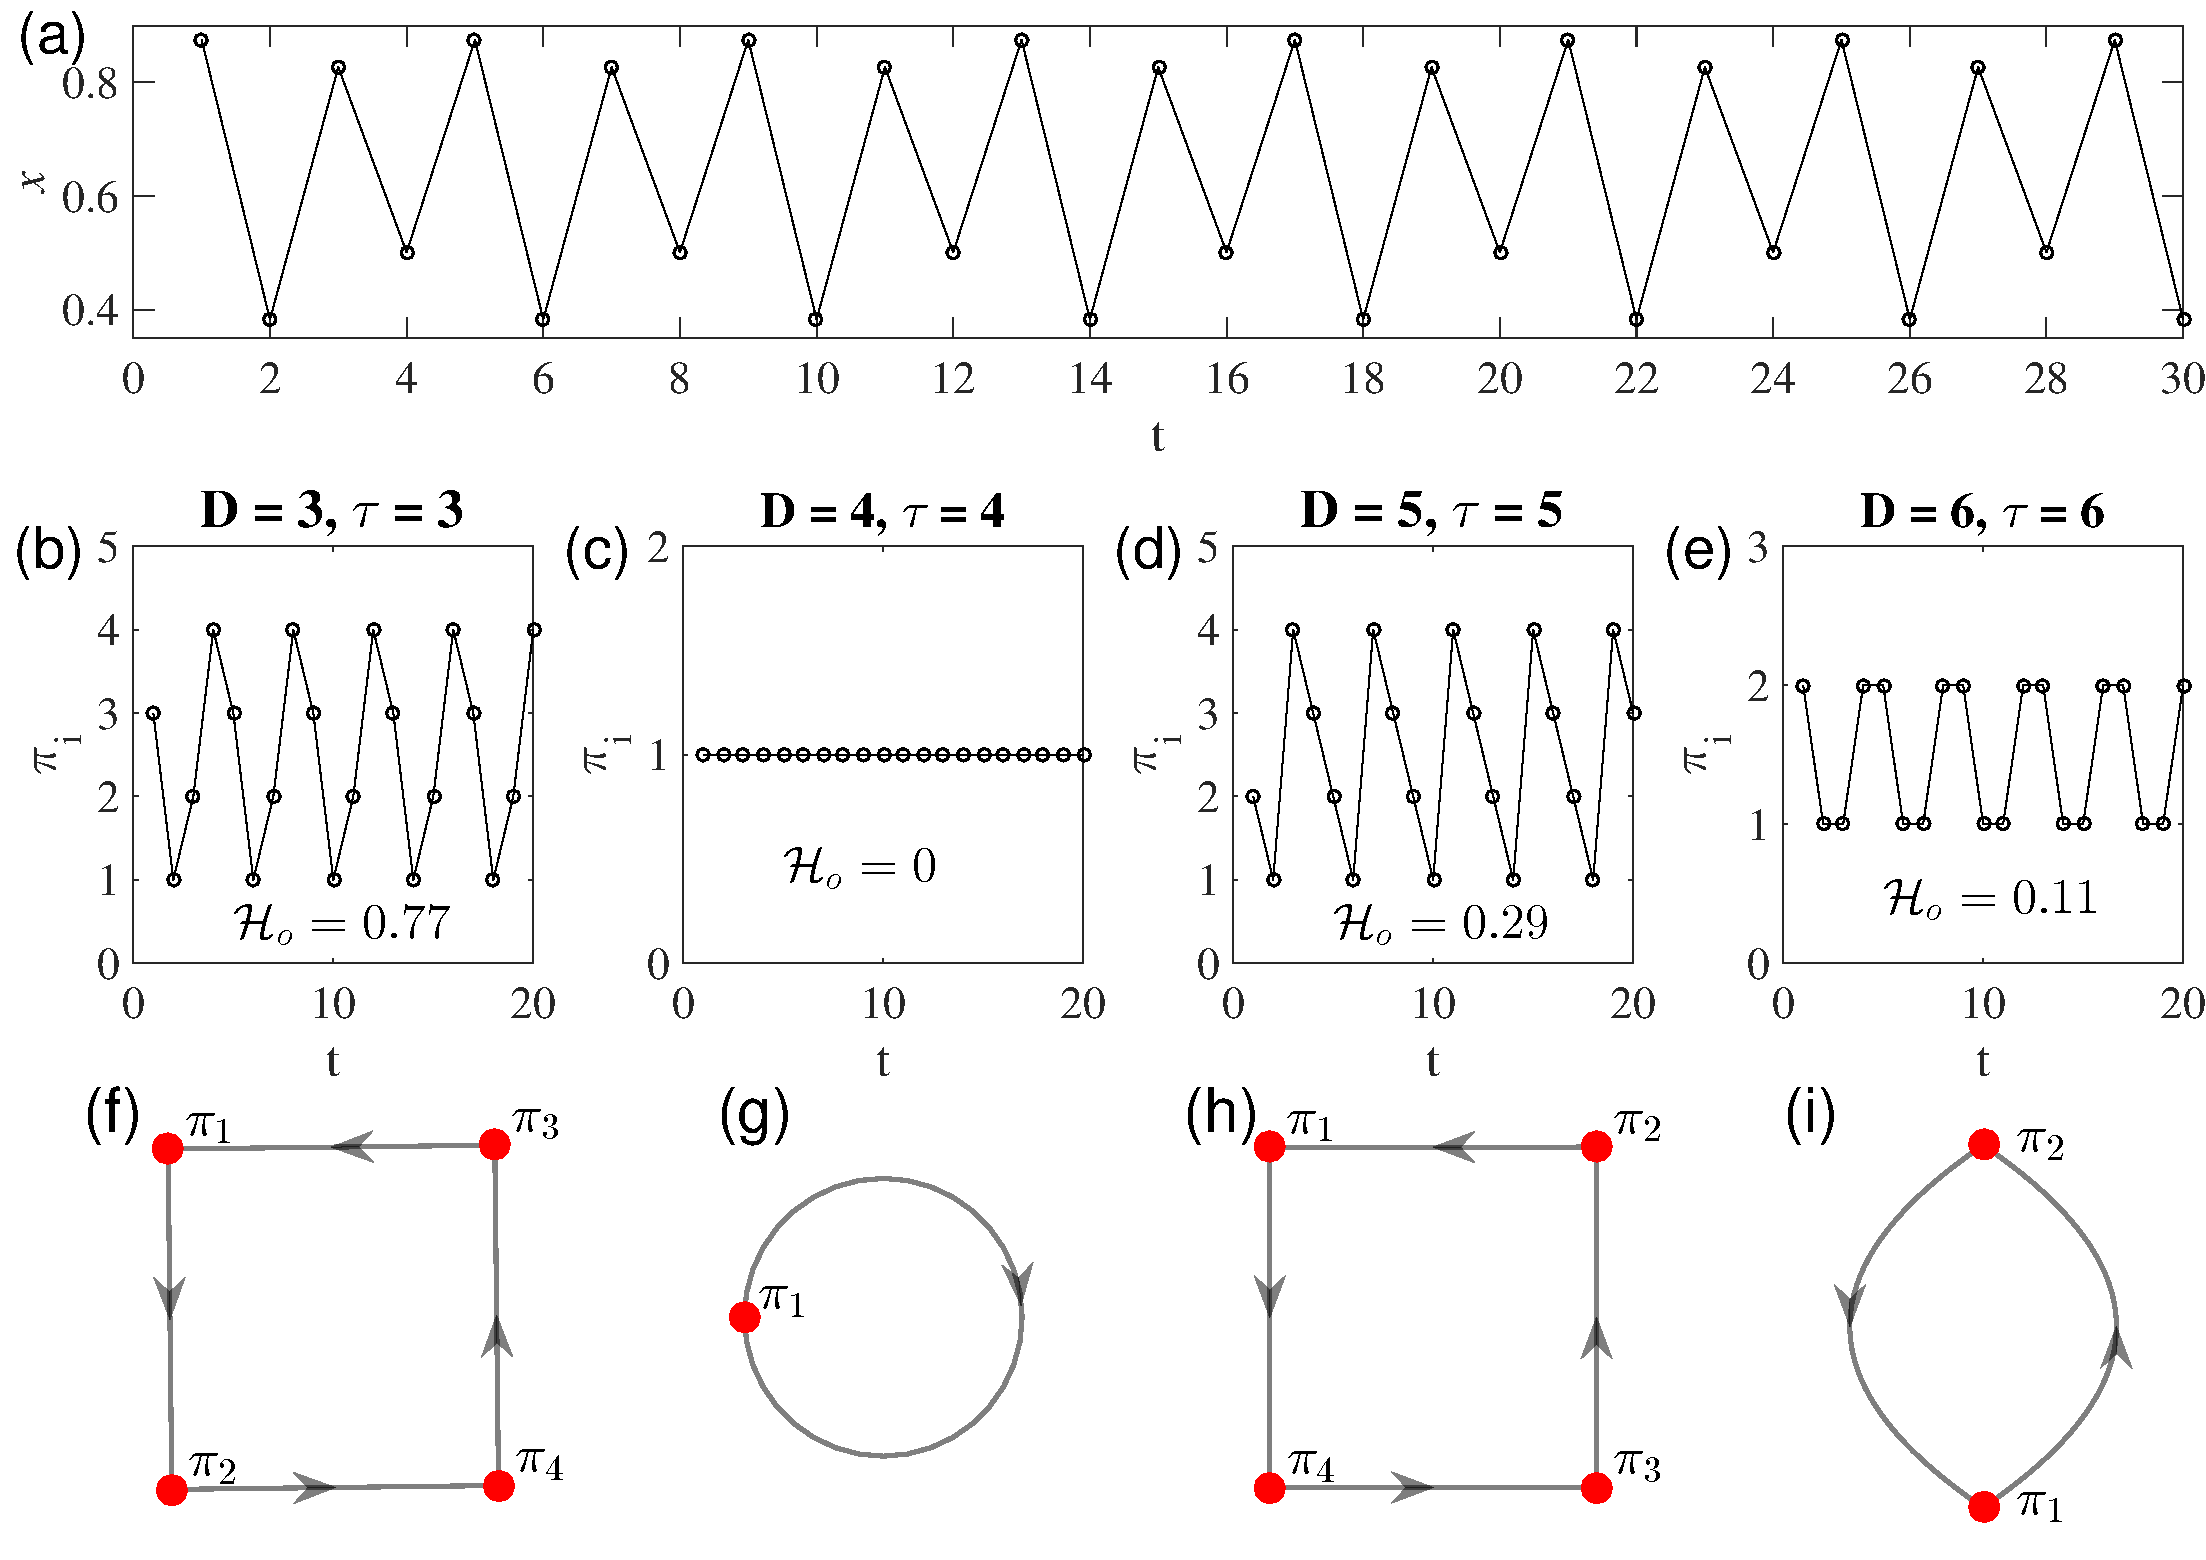
\includegraphics[width=2\columnwidth]{period4_logisticExample.pdf}
\caption{\small{Example of a period-4 time series demonstrating the effects of different choices of the embedding parameters $D$ and $\tau$. (a) Time series comprising 30 iterations of the period-4 orbit. The corresponding ordinal pattern series are shown for different combinations of $D$ and $\tau$ \textcolor{red}{selected for illustrative purposes}: (b) $\tau = D = 3$, (c) $\tau = D = 4$, (d) $ \tau = D = 5$, and (e) $\tau = D = 6$. The respective permutation entropy values normalized by $\log D!$ as in Eq.~\eqref{eq:Ho} are indicated in the insets of each panel. Panels (f)-(i) show the corresponding OPTNs. The weights of directed edges are not shown (recall that two slightly different normalizations are considered in this work). Note that in panel (g), there exist exclusively self-loops since $\tau = D = 4$ results in a unique, constant pattern. Missing patterns are suppressed.}
\label{fig:embed}}
\end{figure*}

As an illustrative example highlighting the important roles of $D$ and $\tau$ for ordinal pattern based \textcolor{red}{time series} analysis, we consider a period-4 solution of the logistic map 
\begin{equation}
x_{i+1}=rx_i(1-x_i) 
\end{equation}
\noindent
with $r= 3.5$. {\color{red}In this example, the choice of $\tau = D$ reflects the particular role of specific choices of the embedding parameters in the context of low-order periodic windows (here, period-4 and period-3) in the bifurcation sequence of the logistic map. As expected,} Fig.~\ref{fig:embed} demonstrates that the resulting ordinal pattern sequences are significantly affected by the different parameter settings, which further result in different permutation entropy values $\mathcal{H}_O$. For instance, only one unique ordinal pattern is observed when $\tau = D = 4$ (Fig.~\ref{fig:embed}(c, g)) resulting in $\mathcal{H}_O = 0$, which is due to the coverage of exactly one full period by the particular embedding parameters. Other values of $D$ and $\tau$ however yield non-zero entropy values. The results of Fig.~\ref{fig:embed} may raise concern since different choices of $D$ and $\tau$ will change the placement of the system in the complexity--entropy plane. %{\color{red}, which is an open problem for ordinal pattern analysis \cite{AmigoPTRSA2014,Riedl2013}.} 
In the special case of the logistic map, we do not have a unique choice of $D$ and $\tau$ for {\color{red}all different} periodic windows when the control parameter $r$ is varied. When the control parameter $r$ is changed, we should \textcolor{red}{rather} focus on the transitions between different dynamical regimes. 
% In the following, we will show that the results are robust when the control parameter is systematically changed while keeping the same embedding parameters. 

\subsection{Results for four typical dynamical regimes} \label{sec:four}
We further illustrate the potential of the proposed SCMs to characterize the logistic map with the control parameter $r$ varying in the range $[3.5, 4]$ with a step size of $\Delta r = 0.001$. In this range of $r$, various dynamical regimes and transitions between them can be found, for instance, period doubling cascades, band merging points, inner and outer crises, and intermittency \cite{Kantz97}, which has made this system serving as a paradigmatic model for assessing nonlinear time series analysis methods \cite{MarwanPLA2009}. 

As a first step, we consider four representative regimes that can be observed at particular values of the control parameter $r$, corresponding to either periodic dynamics or chaotic dynamics close to band merging, in some laminar state, and at the outer crisis. In all examples, we will consistently use the embedding parameters $D = \tau = 6$. 
%In general, we emphasize that a higher value of $D$ leads to a larger variety of ordinal patterns and, hence, a more robust statistics. On the other hand, for evaluating the statistical properties of either pattern frequencies or transition frequencies, this comes on the cost of requiring increasingly longer time series. 
In the following, we will use realizations of the logistic map comprising $L = 10^6$ iterations (after removing the first $1000$ iterations of each realization which might reflect transient behavior of the system before reaching its respective attractor)\textcolor{red}{, which meets the conditions for the necessary time series length for $D=6$ as discussed in Sect.~\ref{sec:tslength}}. 

For all four situations, we investigate the SCMs along with their dual entropy characteristics in detail and summarize the obtained results in Tab.~\ref{tableLog}. We note that several types of chaos--chaos transitions will be discussed in the following: the band merging crisis corresponds to intermittency, the inner crisis to some more subtle chaos-chaos transition and the outer crisis to fully chaotic dynamics. 
\begin{table}[htb]
    {\begin{tabular}{l  l  l  l  l  l  l  l}
    \hline
    Regime & $r$      & $\mathcal{H}_O$ & $\mathcal{C}_O$ & $\mathcal{H}_W$ & $\mathcal{C}_W$ & $\mathcal{H}_E$   & $\mathcal{C}_E$  \\
    \hline
    period-3      & 3.83 & 0 & 0 & 0 & 0 & 0 & 0 \\
    \hline
    band merging    & 3.679 & 0.978 & 0.043 & 0.639 & 0.582 & 0.302 & 0.277  \\
    \hline
    laminar state    & 3.791 & 0.989 & 0.026 & 0.671 & 0.618 & 0.354 & 0.328 \\
    \hline
    outer crisis  & 4.0 & 1.0 & 0 & 0.761 & 0.662 & 0.522 & 0.458 \\
    \hline
    \end{tabular}}
   \caption{Values of the three considered SCMs along with their adjoint entropy measures for four different values of the control parameter $r$ of the logistic map (embedding parameters: $D = \tau = 6$).   \label{tableLog}}    
\end{table}

Due to our choice of $\tau$ and $D$, all SCMs take values of zero for the period-3 series because the temporal distance between each pair of components of the embedding vector covers a multiple of two full periods (cf.~Fig.~\ref{fig:embed}). Other choices of $D$ and $\tau$ would commonly yield non-zero values for the period-3 regime. For the three other cases of band merging, laminar state and outer crisis, the values of all SCMs significantly differ from zero. The pattern frequency based SCM $\mathcal{C}_O$ shows zero value and $\mathcal{H}_{O} = 1$, which implies a positioning in the lower right corner of the complexity--entropy plane in Fig.~\ref{fig:CElogistic}(a). However, for the transition matrix based SCMs, both the estimated entropies $\mathcal{H}_W$, $\mathcal{H}_E$ and associated complexity measures $\mathcal{C}_W$, $\mathcal{C}_E$ show results that are more consistent with the expectations when considering the respective level of chaoticity of the system in those three regimes (i.e., a rising Lyapunov exponent with increasing $r$ in the respective chaotic regimes). In particular, the estimated SCMs take their largest values for $r = 4$ in the outer crisis regime, and the SCMs are the smallest when $r = 3.679$ in the band merging case, while the laminar regime displays intermediate SCM values. 

\subsection{Complexity--entropy planes} \label{sec:plane}
\subsubsection{Logistic map} 
In order to put our previous results into a broader context, we next show the complexity--entropy planes obtained when varying the control parameter $r$ in the logistic map. This simple nonlinear system has already been widely discussed in the framework of SCMs \cite{RossoPRE2007,MartinPLA2003}, but only for pattern frequency based complexity measures. For each value of $r$, we construct an OPTN from a time series of length $L = 10 ^ 6$ with the embedding parameters $D = \tau \in \{2,\ldots,7\}$. 

As already stated above, when only one unique ordinal pattern is identified in a given time series, all SCMs take a value of $0$, which is reasonable since only self-loops are observed. This however happens only if the embedding parameters are chosen such that they exactly coincide with the periodicity of a certain periodic window (see Fig.~\ref{fig:embed}(g)). 
%Another practical aspect concerns the data requirements for computing entropies and complexity measures. For a reliable estimation of SCMs, a pragmatic condition on the length $L$ of the time series to be sufficiently larger than $D!$ \cite{rossoPRL2007,kowalskiPhyD2007} has been satisfied in our setting for $D \leq 7$. In the particular example of the logistic map, one may easily generate much longer realizations, which however {\color{red} is subjected to finite size effects in experimental time series analysis}. 

In previous works, SCMs have been applied to distinguish chaos from noise by employing the concept of complexity--entropy plane~\cite{rossoPRL2007}. Generalizing this idea to our OPTN based SCMs, we can define three such planes showing the statistical complexity measures ($\mathcal{C}_O$, $\mathcal{C}_W$ and $\mathcal{C}_E$) as a function of the corresponding normalized entropy values ($\mathcal{H}_O$, $\mathcal{H}_W$ and $\mathcal{H}_E$). The three SCMs characterize both randomness and correlation structure in a time series, which as a consequence result in a non-trivial dependence on the associated entropy values. Specifically, chaotic systems present high complexity while stochastic systems have lower values of complexity, hence ideally appearing in distinct regions of the complexity--entropy plane~\cite{rossoPRL2007}. Furthermore, {\color{red}it has been shown previously that at a given entropy value,} the range of possible SCM values is bound by a minimum $\mathcal{C}_{min}$ and a maximum $\mathcal{C}_{max}$. A general algorithm for computing these bounds has been provided in Ref.~\cite{martinPhyA2006}. 

Figure~\ref{fig:CElogistic} shows the complexity--entropy planes for embedding parameters $D = \tau$ varied between $4$ and $6$. We emphasize that the results are qualitatively similar when $D$ and $\tau$ are varied in the range $\{3,\ldots, 7\}$. Furthermore, it is notable that the values of $\mathcal{C}_{max}$ depend on the embedding dimension $D$ since $D$ determines the number of patterns and pattern transitions which are considered in the definition of SCMs. {\color{red}The curves of $\mathcal{C}_{max}$ for different embeddings have been further annotated in Fig. \ref{fig:CElogistic}. In contrast, the $\mathcal{C}_{min}$ values are close to each other, showing less dependence on $D$, and therefore they are not annotated. }
\begin{figure*}
	\centering 
	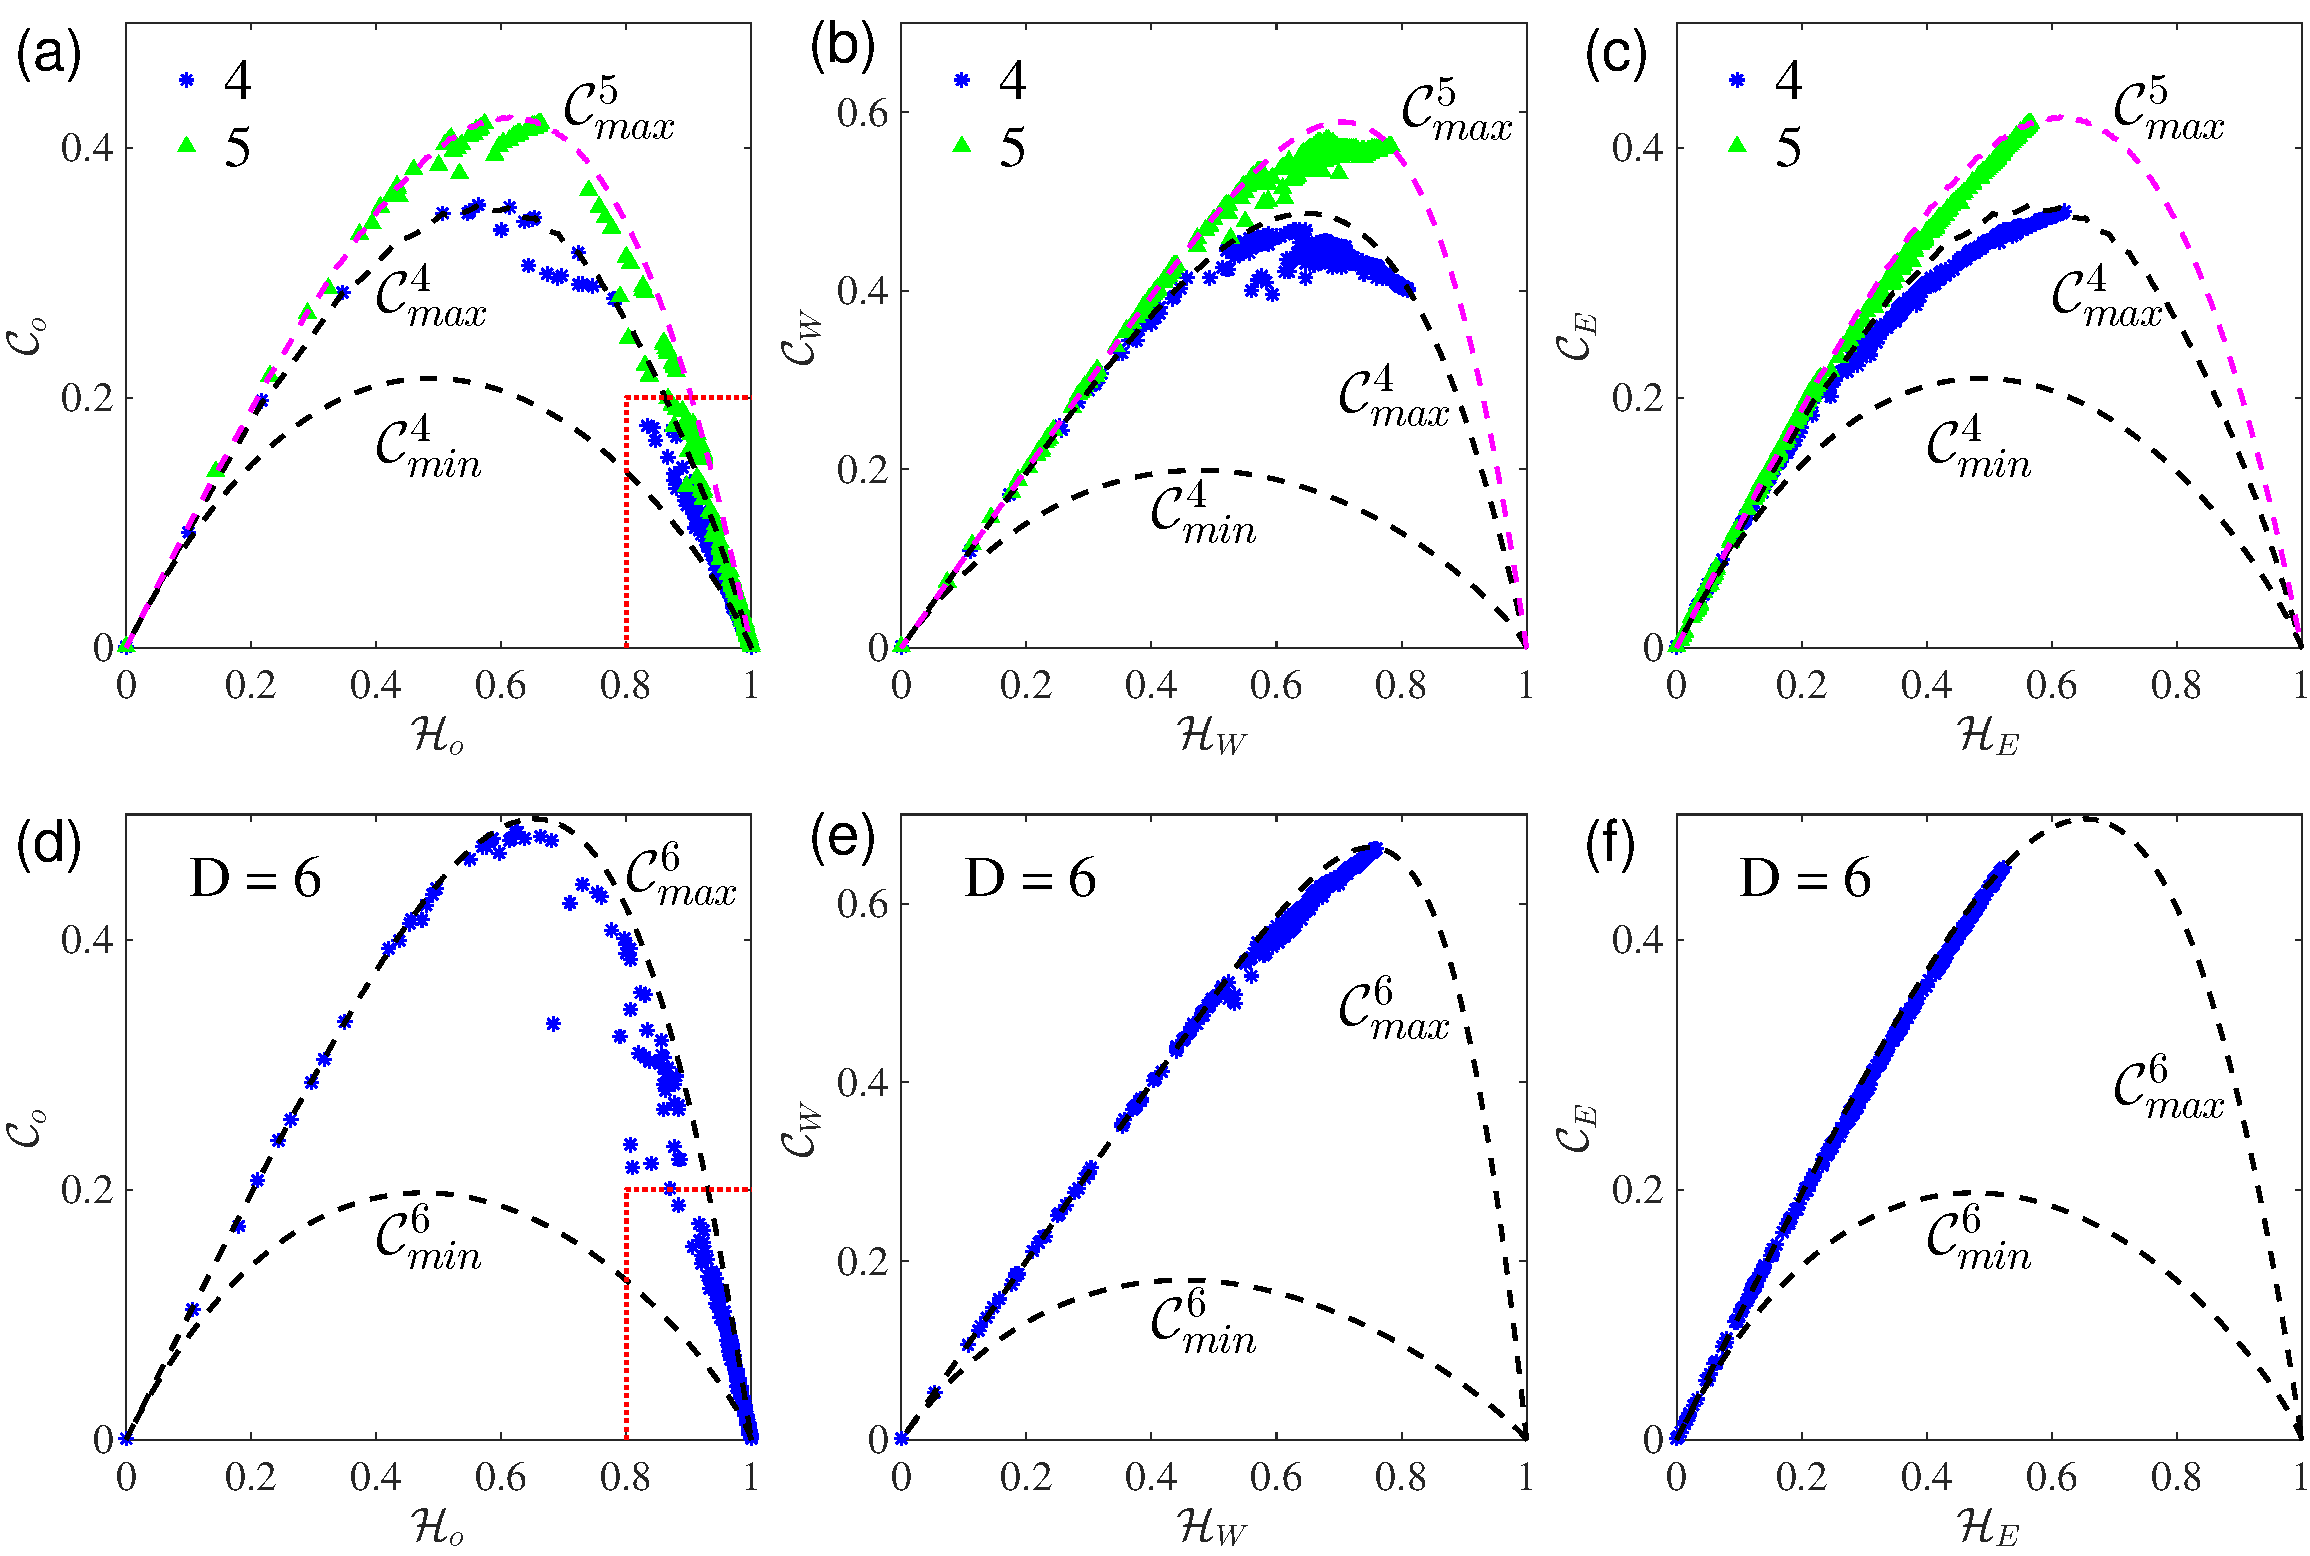
\includegraphics[width=2\columnwidth]{CompEntropy_LogisticHC.pdf}
\caption{\small{(Color online) Three different complexity--entropy planes (based on the Jensen-Shannon divergence) illustrating the behavior of the three SCMs for example series of the logistic map with varying control parameter $r$: (a, d) $\mathcal{C}_O$ versus $\mathcal{H}_O$, (b, e) $\mathcal{C}_{W}$ versus $\mathcal{H}_{W}$, and (c, f) $\mathcal{C}_{E}$ versus $\mathcal{H}_{E}$. The {\color{red} dotted lines correspond to $\mathcal{C}_{max}$ and $\mathcal{C}_{min}$ in dependence on the respective entropy for $D=4$, and the dashed lines are $\mathcal{C}_{max}$ and $\mathcal{C}_{min}$ for $D=5$. Panels (a-c) show the results for embedding dimensions $D = 4,5$ with annotations for the respective $\mathcal{C}_{max}$ only} and (d-f) for $D = 6$. In panels (a, d), the bottom-right rectangles of dotted red lines indicate the regions for the traditional pattern frequency based SCM analysis where the differentiation between stochastic and deterministic--chaotic dynamics is ambiguous. However, the lower left rectangles of (b, c, e, f) correspond to regions of lower complexities. }  \label{fig:CElogistic}}
\end{figure*}

First of all, we recover the known result that pattern frequency based SCM values lie close to the maximum $\mathcal{C}_{max}$, while the displacements of the estimated values from their theoretical upper bounds depend on the embedding dimension $D$ as shown in Fig.~\ref{fig:CElogistic}(a,d). Most notably, we find many combinations of complexity--entropy values in the lower right part of the plane (high entropy, low complexity), which have been highlighted by rectangles of dotted lines. This region of the plane is challenging for SCMs to distinguish between chaotic time series and random noise~\cite{BorgesAMC2019} and is in our case occupied by values corresponding to chaotic regimes of the logistic map at large $r$ values. The corresponding ambiguity results from the fact that both $\mathcal{H}_O$ and $\mathcal{C}_O$ only take static information in the sense that only pattern frequencies have been considered in their definitions. 

For our new pattern transition based SCMs, we find that in the complexity--entropy planes $\mathcal{H}_W \times \mathcal{C}_W$ and $\mathcal{H}_E \times \mathcal{C}_E$, the results for the logistic map again closely align with the theoretical upper bounds $\mathcal{C}_{max}$. When increasing the embedding dimension, the estimated values approach the theoretical $\mathcal{C}_{max}$ curve more and more closely and essentially cover exclusively the left uprising branch of the curve for the SCM based solely on transition frequencies (Figs.~\ref{fig:CElogistic}(b, e) and \ref{fig:CElogistic}(c, f)), which distinctively differs from the original permutation entropy based SCM. Specifically, the definition of $\mathcal{C}_{E}$ and $\mathcal{H}_{E}$ takes information on both, pattern frequencies and transition frequencies into account, which results in the obtained SCM values aligning even more closely with $\mathcal{C}_{max}$ already at lower embedding dimensions (Fig.~\ref{fig:CElogistic}(c, f)). In our opinion, the most interesting result is, however, that we do not find any values in the lower right part of the plane, which for the classical SCM based on permutation entropy would present the challenging region of possible ambiguity between deterministic-chaotic and stochastic dynamics. 

{\color{red}On the other hand, there are many values in the lower left corner of the plane showing small values of $\mathcal{C}_{W}$ and $\mathcal{C}_{E}$ (Fig. \ref{fig:CElogistic}(b, c, e, f)). This region corresponds to regular orbits of low complexities. Along with the choice of embedding parameters, the length of time series and long term accumulations of the computation precisions play important roles in the lower left region of the complexity planes, which will be further further discussed in Sec. \ref{sec:transi}. Out of the left and right corners, complexities of $\mathcal{C}_{W}$ and $\mathcal{C}_{E}$ show consistent trends along with the degree of chaoticity as will be explained later in Sec. \ref{sec:transi}.} In general, we therefore suggest that it is the deterministic transition behavior among patterns that allows an improved distinction from random noise. 

{\color{red}In addition, we observe a linear correlation between $\mathcal{C}_W$ and $\mathcal{H}_{W}$ (Fig. \ref{fig:CElogistic}(e)), respectively, $\mathcal{C}_{E}$ and $\mathcal{H}_{E}$ (Fig. \ref{fig:CElogistic}(f)). However, we note that this linear correlation appears only for large embedding $D = 6$ and coincides with the up-rising brach of the maximal complexity curve $\mathcal{C}_{max}$, which is expected by the theory \cite{SMCbook2010}.}

{\color{red} The discriminatory power of different SCMs have been further compared in Fig. \ref{fig:CHlogCmax}, which characterize how well the alignments are to the maximal complexity $\mathcal{C}_{max}$. In particular, for a given $\mathcal{H}$ we compute a normalized complexity $\mathcal{C}^{N} = (\mathcal{C} - \mathcal{C}_{min}) / (\mathcal{C}_{max} - \mathcal{C}_{min})$. In consequence, $\mathcal{C}^{N}$ is bounded in the interval of $[0, 1]$ and the alignments along $\mathcal{C}_{max}$ are reflected by large values of $\mathcal{C}^{N}$. The results are shown in Fig. \ref{fig:CHlogCmax}. For the traditional $\mathcal{C}_{O}$, again we find there are many points in the right half plane (Fig. \ref{fig:CHlogCmax}(a) for all embedding dimensions. In contrast,  there are no points in the region of $\mathcal{H} >0.8$ for $\mathcal{C}_W$ and $\mathcal{C}_E$ (Fig. \ref{fig:CHlogCmax}(b,c)). Note that in Fig. \ref{fig:CHlogCmax}(c), the dots larger than 1 are numerical artefacts when the control parameters $r$ are close bifurcation points resulting in long transients (as will be explained by Fig. \ref{fig:transient} in Sec. \ref{sec:transi}).  
\begin{figure*}
        \centering
        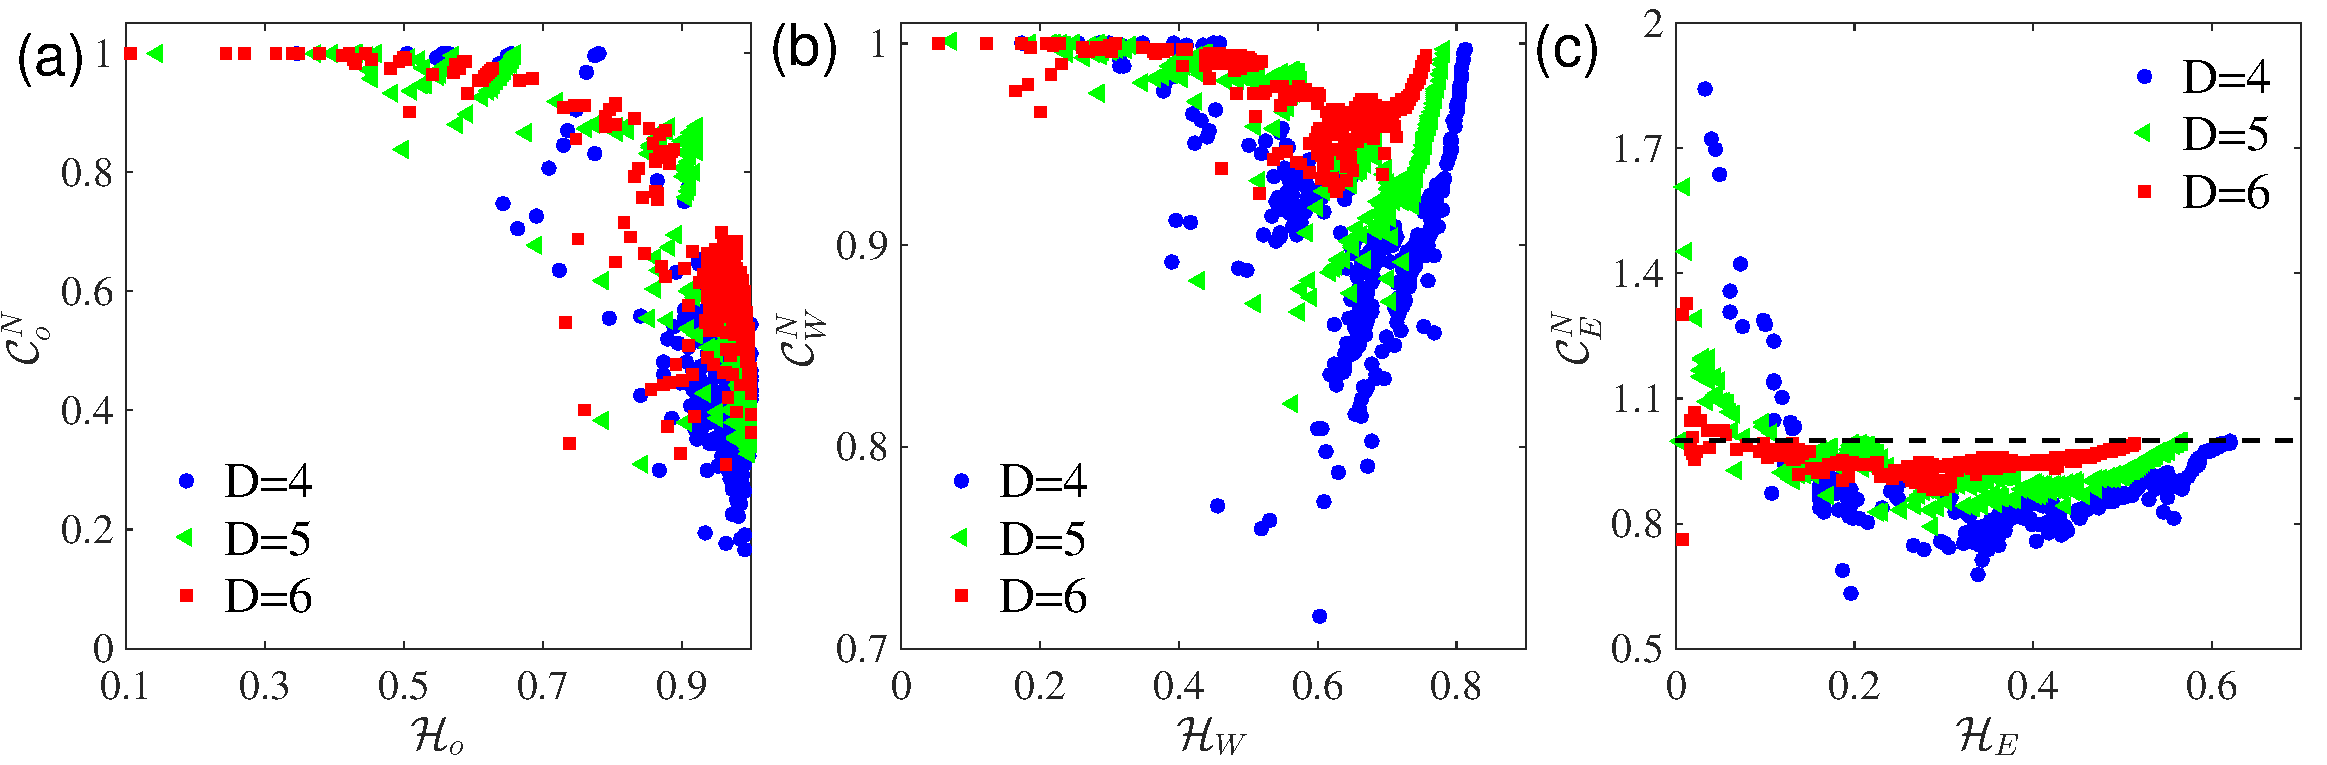
\includegraphics[width=2\columnwidth]{CompEntropyCNormalized_Logistic.pdf}
\caption{(Color online) Normalized complexity -- entropy planes of three SCMs for the logistic map, which are normalized by $\mathcal{C}_{max}$ and $\mathcal{C}_{min}$  at a given $\mathcal{H}$. (a) $\mathcal{C}_O$, (b) $\mathcal{C}_W$, and (c) $\mathcal{C}_E$. In (c), the dots larger than 1 are numerical artefacts when the control parameters $r$ are close bifurcation points resulting in long transients. Embedding dimensions are indicated by legends.  \label{fig:CHlogCmax}}
\end{figure*}
}

\subsubsection{Fractional Brownian motion and fractional Gaussian noise}
In order to further analyze the capability of our modified complexity--entropy planes to distinguish chaotic from stochastic dynamics, we compare the results for the logistic map with those obtained for fractional Brownian motion (fBm), i.e., stochastic processes with long-range temporal correlations. Specifically, for an fBm process the long-range correlations of the process are uniquely characterized by the Hurst exponent $H$ when positively correlated (persistence) for $1/2 < H < 1$, while being suppressed (anti-persistence) for $0< H < 1/2$. $H=1/2$ corresponds to the classical Brownian motion. Similar to the previous case of the logistic map with varying control parameter $r$, we generate time series for varying $H \in (0, 1)$ with a step size of $\Delta H=0.05$ and present the resulting complexity--entropy planes in Fig.~\ref{fig:CEfBm}. Moreover, since fBm series in the persistent regime are nonstationary, we further transform all fBm realizations into stationary time series by employing first-order difference filtering, i.e., by considering the increments $x_{i+1}- x_i$. The transformed series are commonly referred to as fractional Gaussian noise (fGn), and the associated complexity--entropy planes are shown in Fig.~\ref{fig:CEfGn}. Notably, fGn retains the long-range correlations and Gaussian probability density function (PDF) of the underlying fBm process. For a discussion on practical concerns regarding time delay embedding of fBm and fGn processes, we refer to Ref.~\cite{Zou2015}. 
\begin{figure*}
	\centering 
	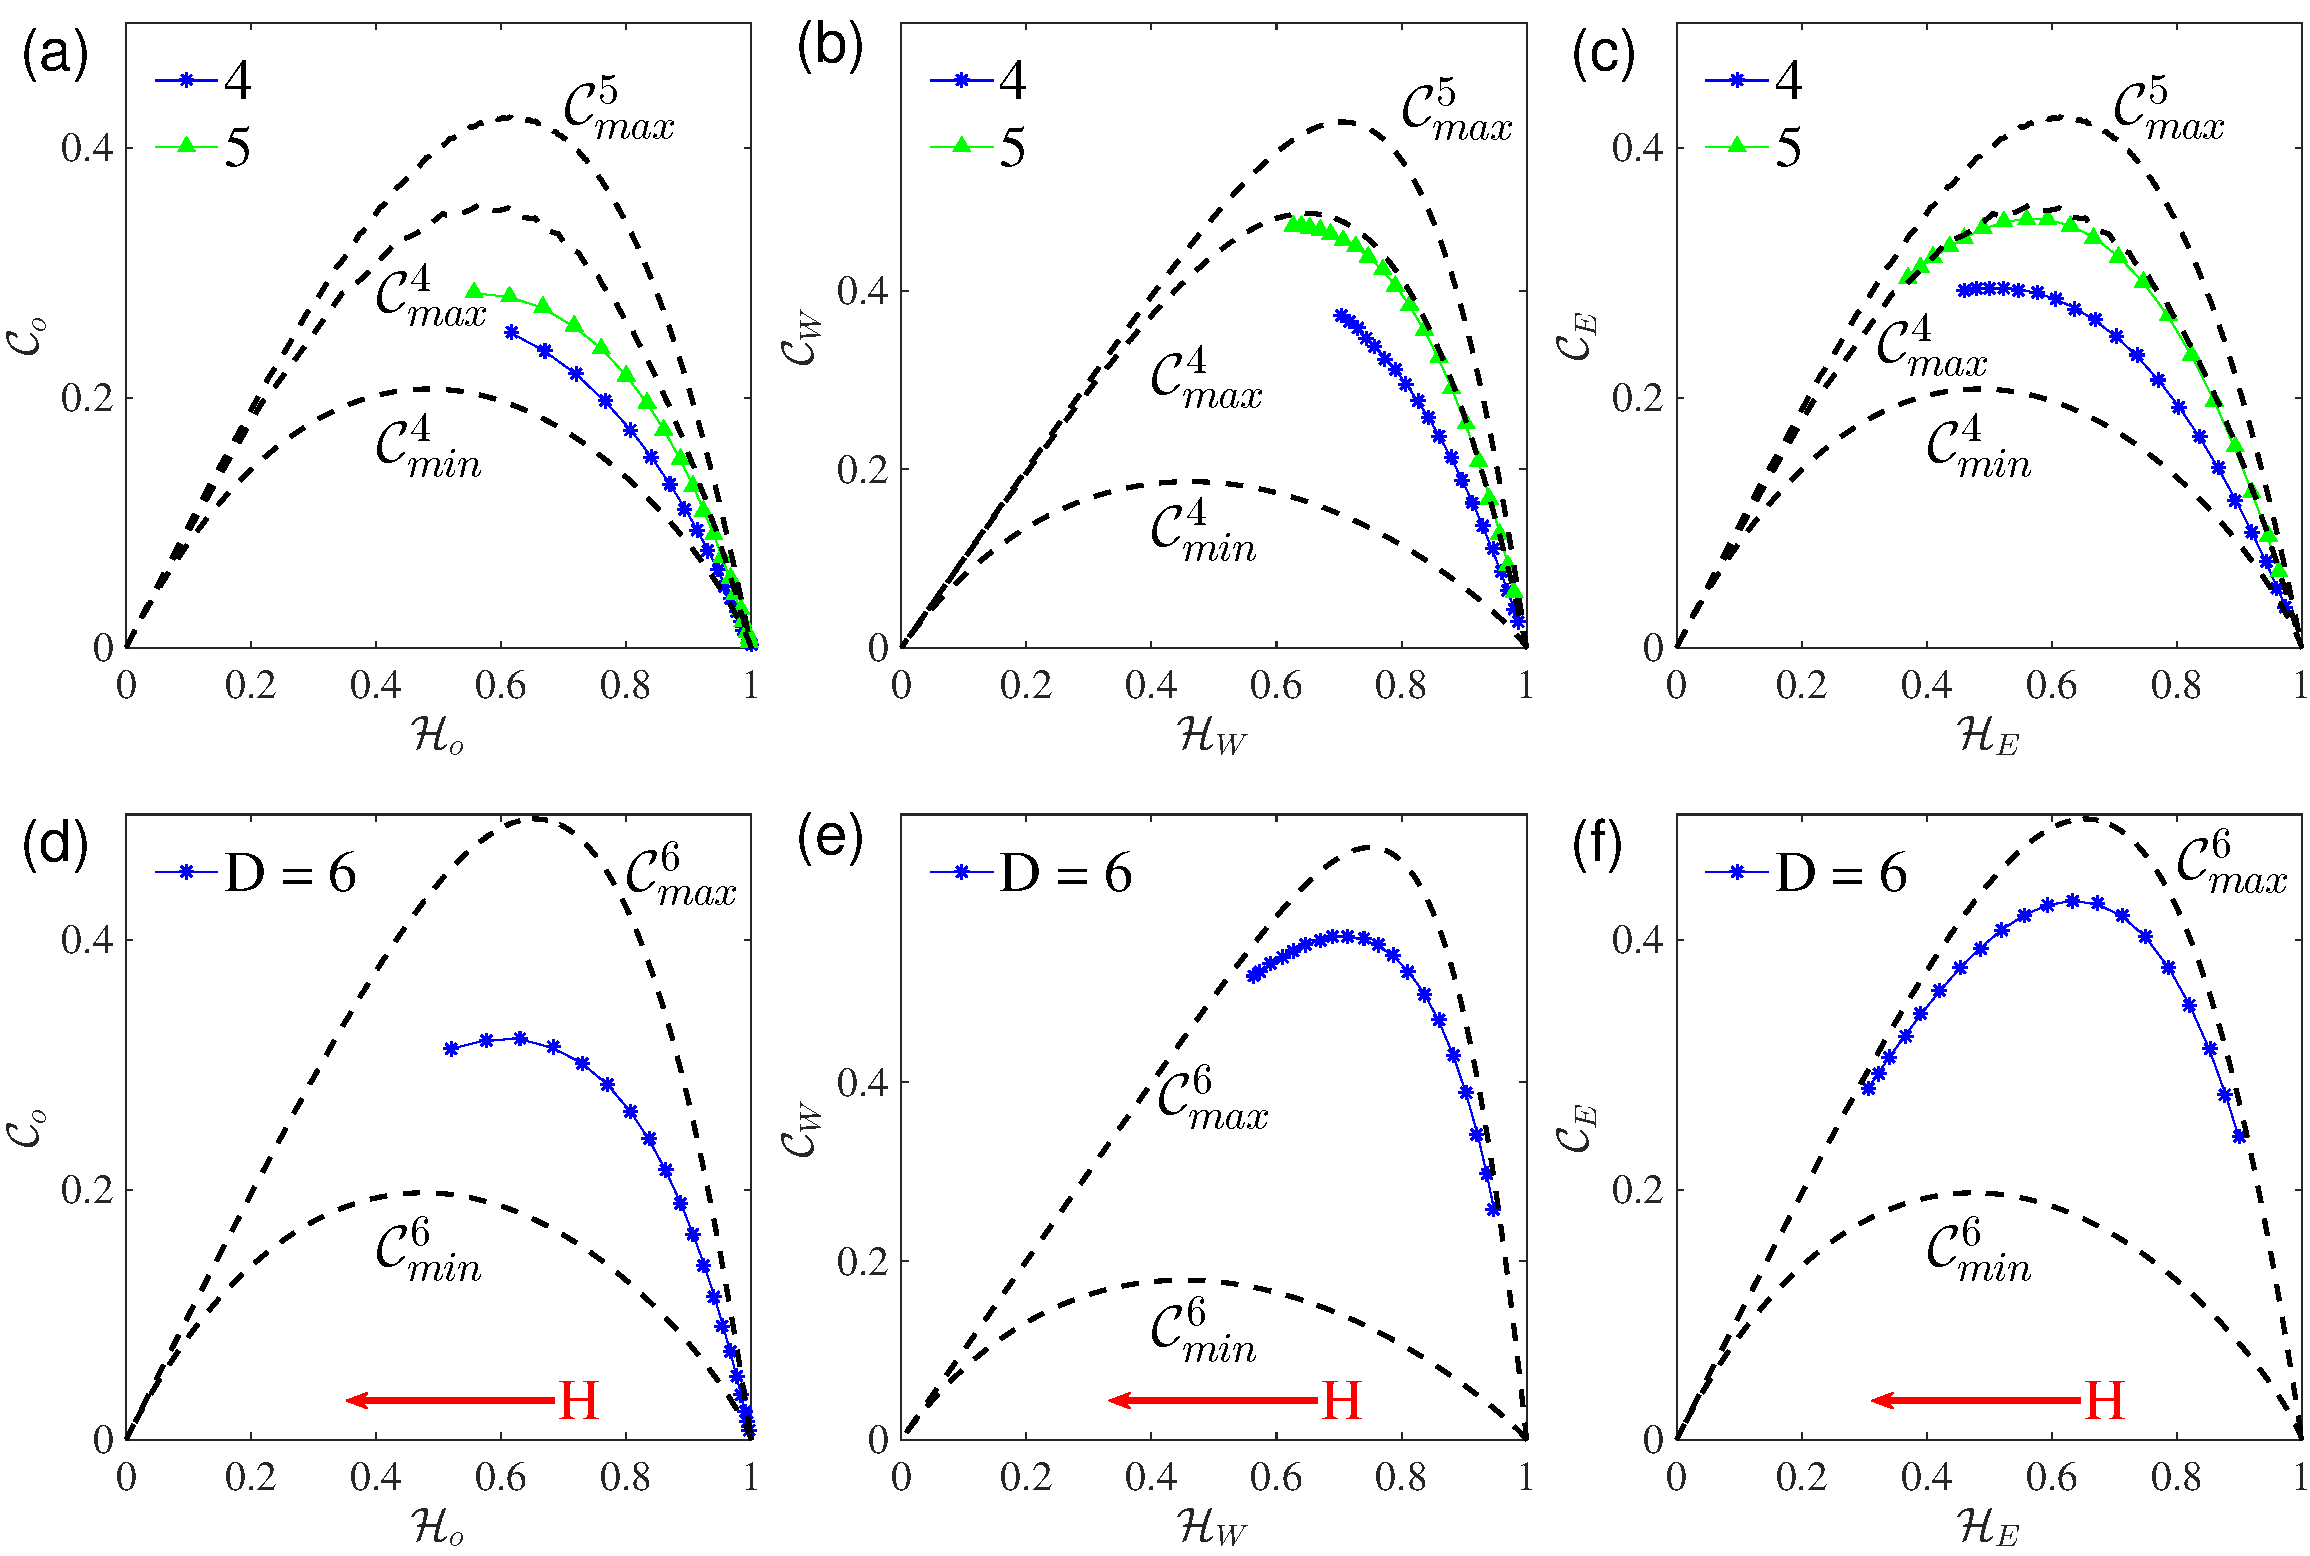
\includegraphics[width=2\columnwidth]{CompEntropy_fBm.pdf}
\caption{\small{(Color online) Same as in Fig.~\ref{fig:CElogistic}, but for fractional Brownian motion with a Hurst exponent $H \in (0, 1)$ varying with a step size of $\Delta H=0.05$. Note that the normalized entropy is generally decreasing with increasing $H$ (red arrow).}  \label{fig:CEfBm}}
\end{figure*}

\begin{figure*}
	\centering 
	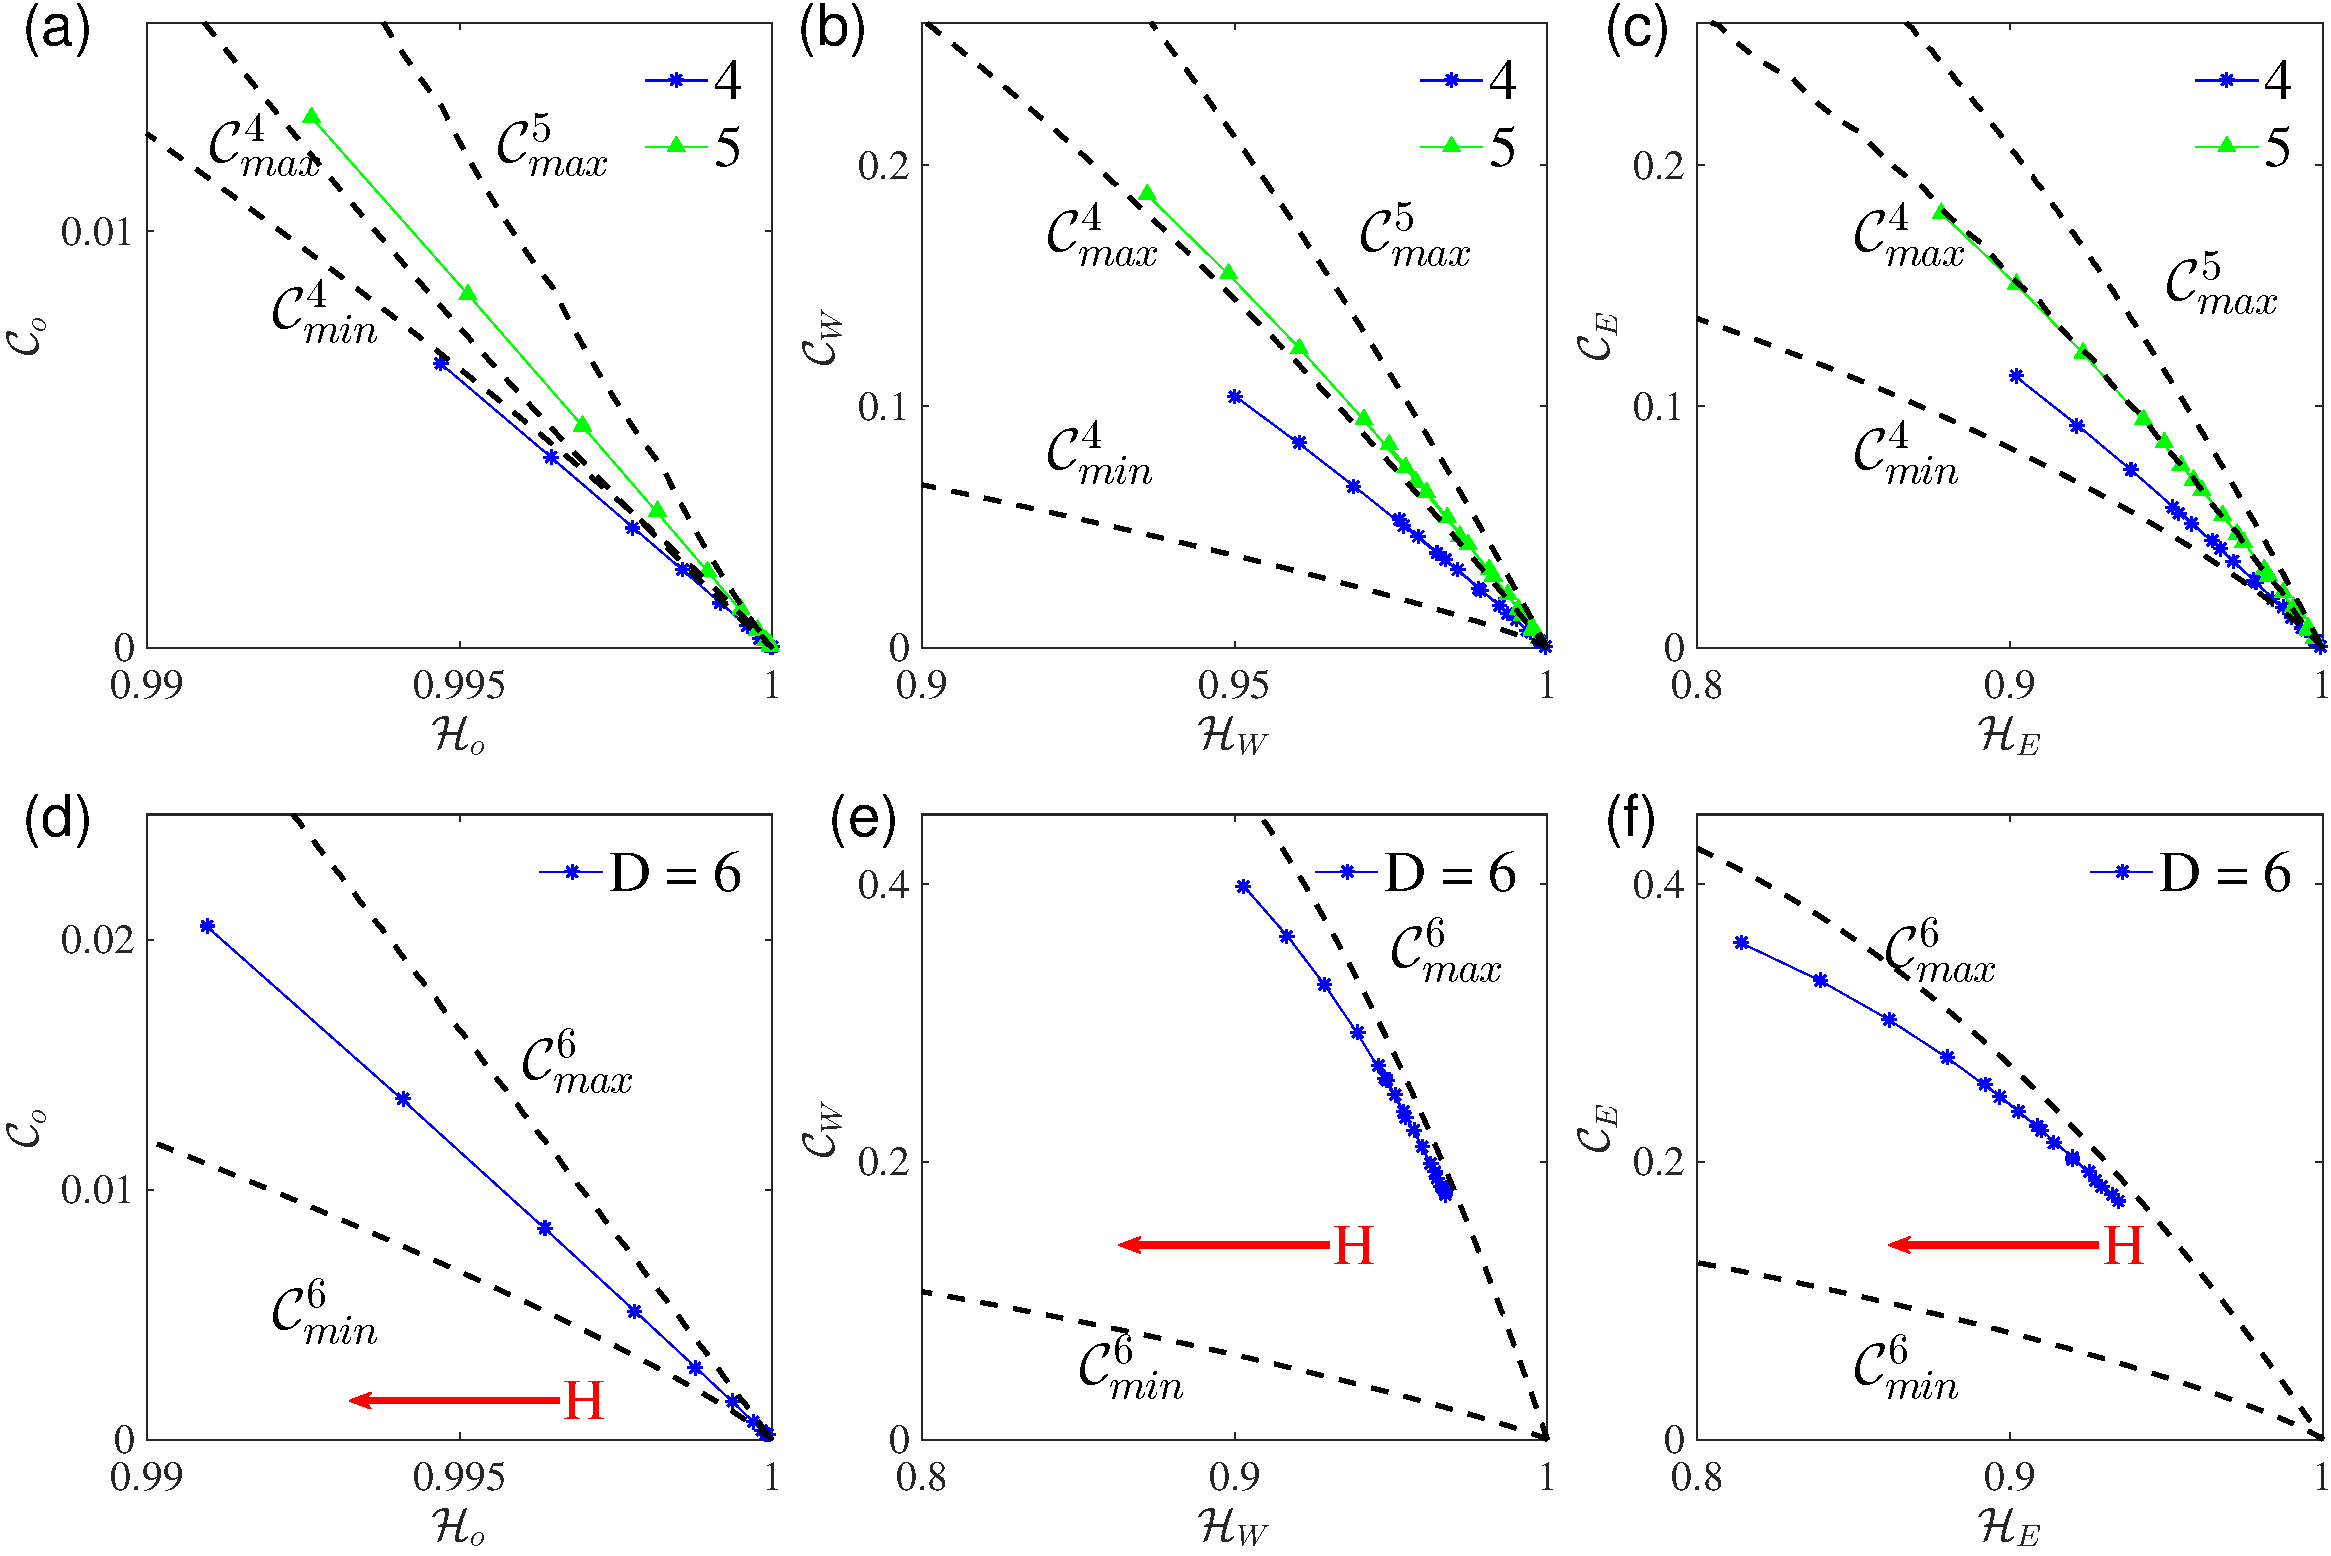
\includegraphics[width=2\columnwidth]{CompEntropy_fGn.pdf}
\caption{\small{(Color online) Same as in Fig.~\ref{fig:CElogistic}, but for fractional Gaussian noise with a Hurst exponent $H \in (0, 1)$ varying with a step size of $\Delta H=0.05$. Note that only a small region of the complexity--entropy planes is covered in this case. }  \label{fig:CEfGn}}
\end{figure*}

{\color{red} For fBM, we show the normalized complexity measures which are obtained by the corresponding $\mathcal{C}_{max}$ and $\mathcal{C}_{min}$ as Fig. \ref{fig:CHfbmCmax}. As the embedding dimension $D$ is increased, the dots are more aligned to $\mathcal{C}_{max}$ and extend further to the left half of the complexity--entropy plane. 
\begin{figure*}
        \centering
        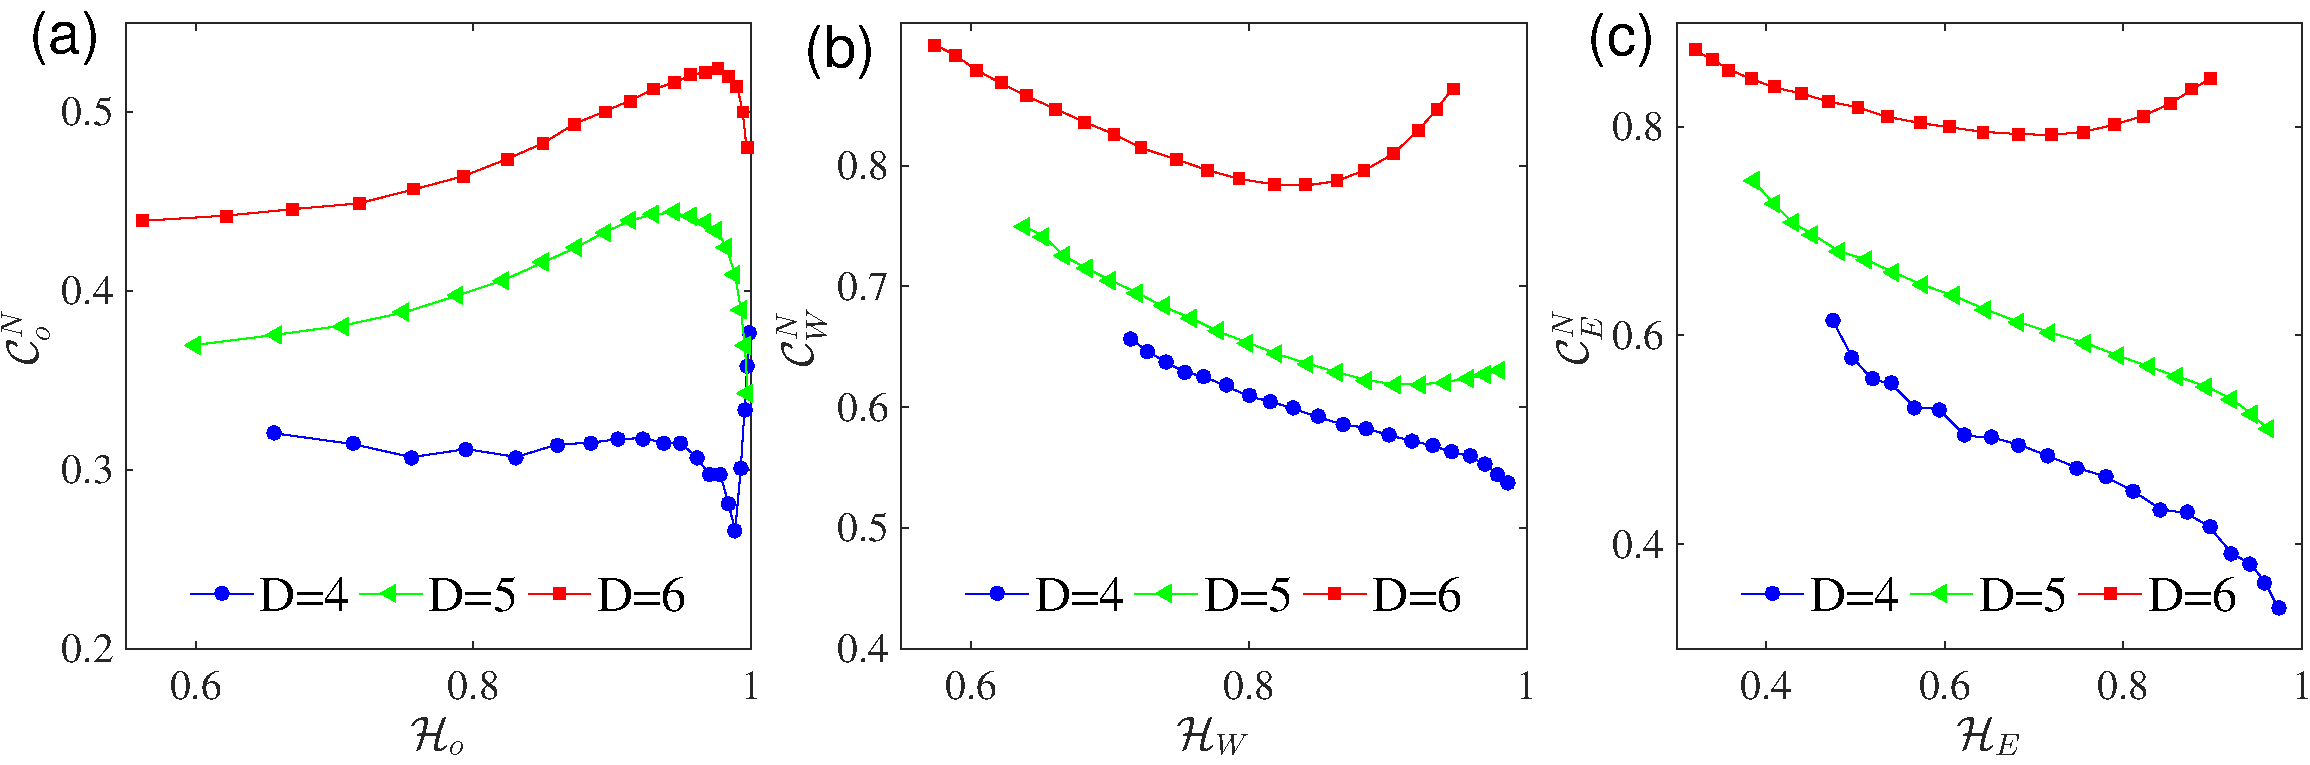
\includegraphics[width=2\columnwidth]{CompEntropyCNormalized_fBm.pdf}
\caption{(Color online) Caption is similar with Fig. \ref{fig:CHlogCmax} for normalized complexity -- entropy planes of three SCMs for the fractional Brownian motion.  \label{fig:CHfbmCmax}}
\end{figure*}
}

Comparing the results for both types of stochastic processes with those for the logistic map, a few important observations are made. First of all, the traditional pattern frequency based SCM values as originally reported by Rosso and co-workers \cite{RossoPRE2007,rossoPRL2007} are well reproduced as expected (Figs.~\ref{fig:CEfBm}(a, d) and \ref{fig:CEfGn}(a, d)). {\color{red}All three pairs of complexity measures lead to parabola-shaped curves as a function of the respective entropy. In addition, the newly proposed complexities of $\mathcal{C}_{W}$ and $\mathcal{C}_{E}$ have higher values, extending to the left plane of lower values for the entropy, which increases chances to discriminate chaos from stochastic processes in comparison to $\mathcal{C}_O$. } 

Second, all complexity--entropy pairs of fBm clearly differ from the theoretical maximum complexity values, which does not change with increasing embedding dimension $D$. Especially for the new OPTN based SCMs, we find a partial overlap between the entropy values of fBm and the logistic map, while the associated SCM values are however clearly distinct except for the cases with the lowest entropy, which correspond to the most nonstationary situations ($H$ close to 1). {\color{red}Taking into account the effects of self loops in the transition matrix, the results of Fig. \ref{fig:CEfBm} do not change significantly although the SCM values extend slightly in the left half of the complexity--entropy plane as $H$ is increased, which are further shown in Fig. S1 of Supplementary Material (SM).} Accordingly, we suggest that combining information on the position in the complexity--entropy plane and on the stationarity could allow a clear distinction between chaotic and stochastic dynamics even in those extreme situations. 

Notably, for the stationary fGn, all entropy measures are confined to very high entropy and low complexity values -- a range where no combinations have been found for the new transition frequency based SCMs for the logistic map. {\color{red}Furthermore, almost the same complexity--entropy plane has been obtained when self loops are included, which has been shown in Fig. S3 of SM. }

Taken all reported results on the complexity--entropy planes for the logistic map, fBm and fGn together, we conclude that the modified SCMs indeed allow distinguishing chaotic from stochastic dynamics more precisely than the original approach. We therefore suggest that the pattern transition behavior encoded in the OPTNs provides novel insights that can be exploited in terms of SCMs that complement their traditional counterparts. 


\subsection{Characterizing dynamical transitions} \label{sec:transi}
The logistic map experiences a sequence of different types of bifurcations when the control parameter $r$ is systematically increased. However, the corresponding dynamical regimes and regime transitions are not easy to identify from the complexity--entropy planes discussed above. In the following, we therefore explicitly study the dependence of our SCMs on the control parameter $r$. Here, our motivation is to verify whether the normalized entropies and associated SCMs computed from OPTNs are indeed able to detect the dynamical transitions along the complex bifurcation scenarios of the logistic map and hence track qualitative changes in the dynamics, including both period--chaos and chaos--chaos transitions. As a benchmark, we take the associated Lyapunov exponent as an established measure for characterizing the type of dynamics (regular versus chaotic) along with the degree of chaoticity.

\begin{figure*}
	\centering 
	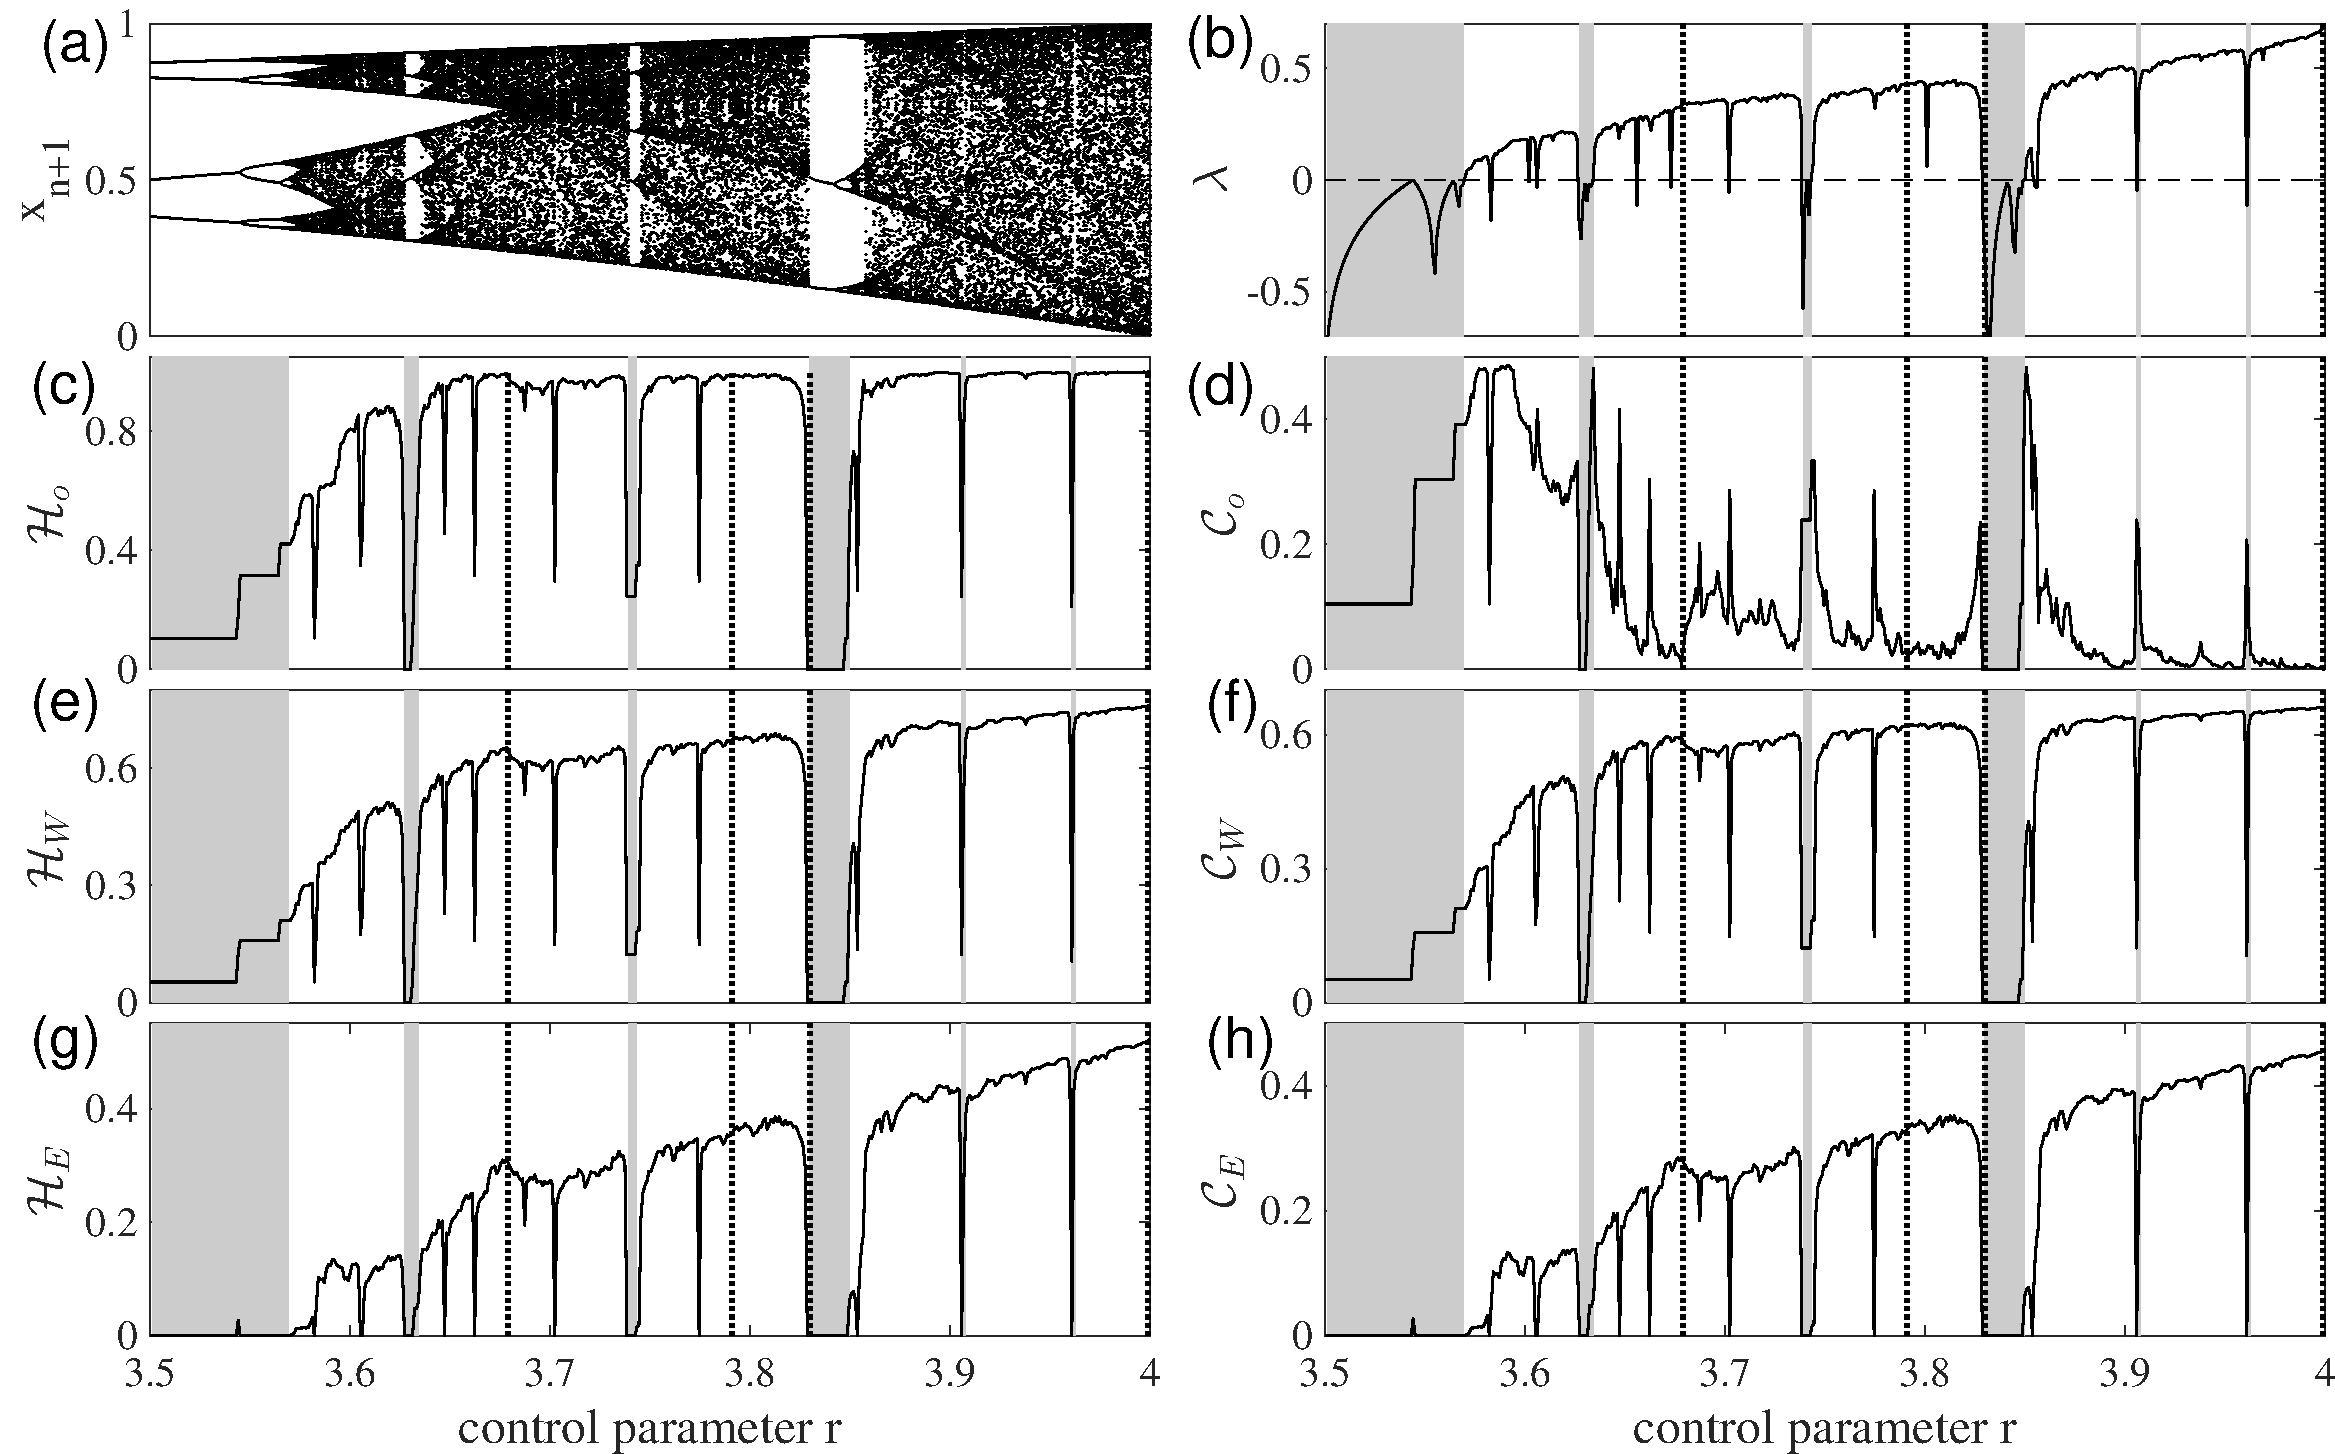
\includegraphics[width=2\columnwidth]{logisticEntropy.pdf}
\caption{\small{Behavior of the different SCMs and associated entropy characteristics for the logistic map in dependence on the control parameter $r$ {\color{red}(embedding dimension $D = 6$).} (a) Bifurcation diagram, (b) Lyapunov exponent, (c) pattern frequency based (permutation) entropy $\mathcal{H}_O$ and (d) associated complexity measure $\mathcal{C}_O$; (e) pattern transition frequency based entropy $\mathcal{H}_W$ based on the globally normalized transition matrix $\mathbf{W}$ and (f) the corresponding complexity measure $\mathcal{C}_W$, and (g, h) entropy $\mathcal{H}_E$ and complexity measure $\mathcal{C}_E$ based on the node-wise out-link normalized transition matrix $\mathbf{W}$. Several major periodic windows have been highlighted by grey background shading. Vertical dotted lines indicate the cases summarized in Tab.~\ref{tableLog}. } \label{fig:bifurcation}}
\end{figure*}

As a general observation, we find that all three SCMs clearly follow the changes in the bifurcation diagram, for instance, showing distinct values in periodic windows (highlighted by grey color in Fig.~\ref{fig:bifurcation}). Other than $\mathcal{C}_O$, the two transition frequency based SCMs behave in a similar way as the Lyapunov exponent. Specifically, as the control parameter $r$ is increased, the chaoticity level grows gradually, reaching a maximum at $r = 4$, which is reflected by an increase in statistical complexity. A similar increase is absent in the pattern frequency based complexity measure $\mathcal{C}_O$ (Fig.~\ref{fig:bifurcation}(c)). In this context, we note that it is an established fact that pattern frequency based SCMs often do not trace the growth in the chaoticity of the logistic map~\cite{MartinPLA2003}, which can however be improved by using Wooter's distance function instead of the Shannon-Jensen divergence employed in this work. From this point of view, the pattern transition frequency based SCMs $\mathcal{C}_W$ and $\mathcal{C}_E$ exhibit some more informative behavior in the sense that they track the growth of the level of chaoticity. 

Another conceptual improvement is found for $\mathcal{H}_E$ and $\mathcal{C}_E$ in the parameter range where the logistic map presents period doubling bifurcations, for example, at $r = 3.544$ (Fig.~\ref{fig:bifurcation}(g, h)). It may be noticed that $\mathcal{H}_O$, $\mathcal{C}_O$, $\mathcal{H}_W$ and $\mathcal{C}_W$ all exhibit non-zero values in this parameter range despite a purely periodic dynamics. Furthermore, there are jumps of all four measures at the points of period doubling bifurcations, which have been already reported in Ref.~\cite{BandtPRL2002}. These jumps however are not desirable since the complexity of the dynamics does not change when $r$ passes any of those points. For the case of the period doubling bifurcation at $r=3.544$ (replacing a period-4 by a period-8 solution), we show in Fig.~\ref{fig:transient} that the observed jump in the entropy and SCM values may be explained by accumulated numerical errors during the iterations attracted to the periodic-4 points, which yields long transients. For estimations based on time series of finite length as used in this work, $\mathcal{H}_E$ and $\mathcal{C}_E$ are however not affected in the same way showing much smaller values (Fig.~\ref{fig:bifurcation}(g, h)). Certainly, we should not over-interpret their capabilities since numerical inaccuracy would be accumulated in a longer iterative process such that different ordinal patterns are identified. In addition, we pass through many periodic windows of different periods as the control parameter $r$ is varied, which prevents us from using a unique predefined number of iterations as initial transients for time series of different period length. Notably, similar jumps have also been observed when the system bifurcates from a period-3 to a period-6 solution at $r = 3.842$. 

\begin{figure}
	\centering
	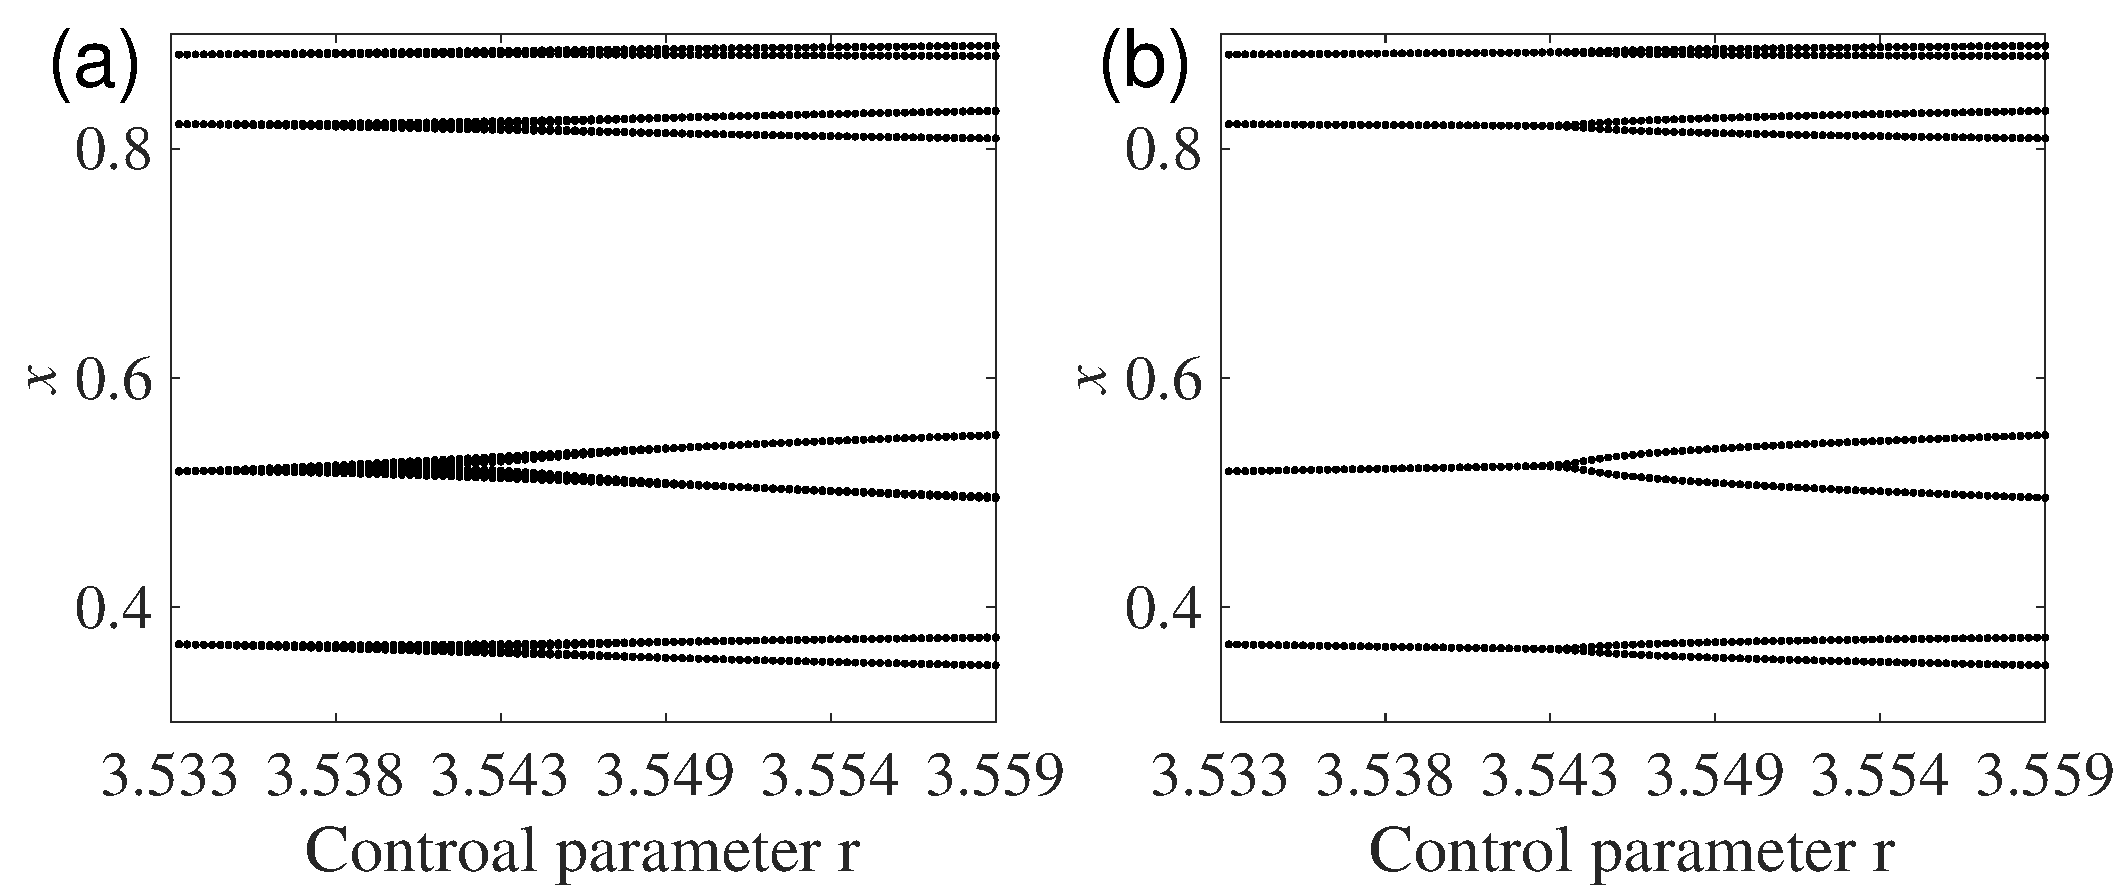
\includegraphics[width=\columnwidth]{period4_exampleTransients.pdf}
\caption{\small{Transient behavior affecting the generation of proper bifurcation diagrams for the logistic map, exemplified here for the period doubling bifurcation from a period-4 to a period-8 solution. (a) The actual bifurcation point gets blurred when $r$ is close to $3.544$ if only a short transient of $50$ iterations is removed from the time series. (b) When a sufficiently large number of initial iterations ($2000$) are removed, the correct bifurcation point becomes visible. }\label{fig:transient}}
\end{figure}

\subsection{Dynamical transitions in continuous system}\label{sec:cont}

While we have focused so far exclusively on the case of the time-discrete logistic map, it may be interesting to study whether a similar behavior can also be obtained for time-continuous deterministic dynamical systems. To this end, we will illustrate a corresponding analysis for the example of the chaotic R\"ossler system \cite{Roessler1976} 
\begin{eqnarray}
\dot{x} &=& -y-z, \nonumber \\
\dot{y} &=& x+0.2y, \\
\dot{z} &=& b+z(x-5.7) \nonumber
\end{eqnarray}
while varying the control parameter $b$. From a conceptual perspective, constructing OPTNs for time series from continuous systems faces certain additional practical challenges, including the proper choice of sampling frequency and embedding parameters, which depend on the particular time scales of the system. To avoid any corresponding discussion on proper choices of further algorithmic parameters, we employ here a Poincar\'e section to each sample trajectory of the system at $y=0$, $\dot{y}<0$ (for different values of $b$) and construct OPTNs from $N = 10,000$ intersection points. The results are shown in Fig.~\ref{fig:bifurRossler}. Based on these results, we conclude that the general behavior of the different SCMs and associated entropy measures closely resembles that reported for the logistic map in Fig.~\ref{fig:bifurcation}. Specifically, all measures trace the succession of bifurcations in the considered range of $b$. We outline more detailed follow-up investigations on the behavior of our OPTN based SCMs to such time-continuous systems directly as relevant topics for future work.

\begin{figure*}
	\centering 
	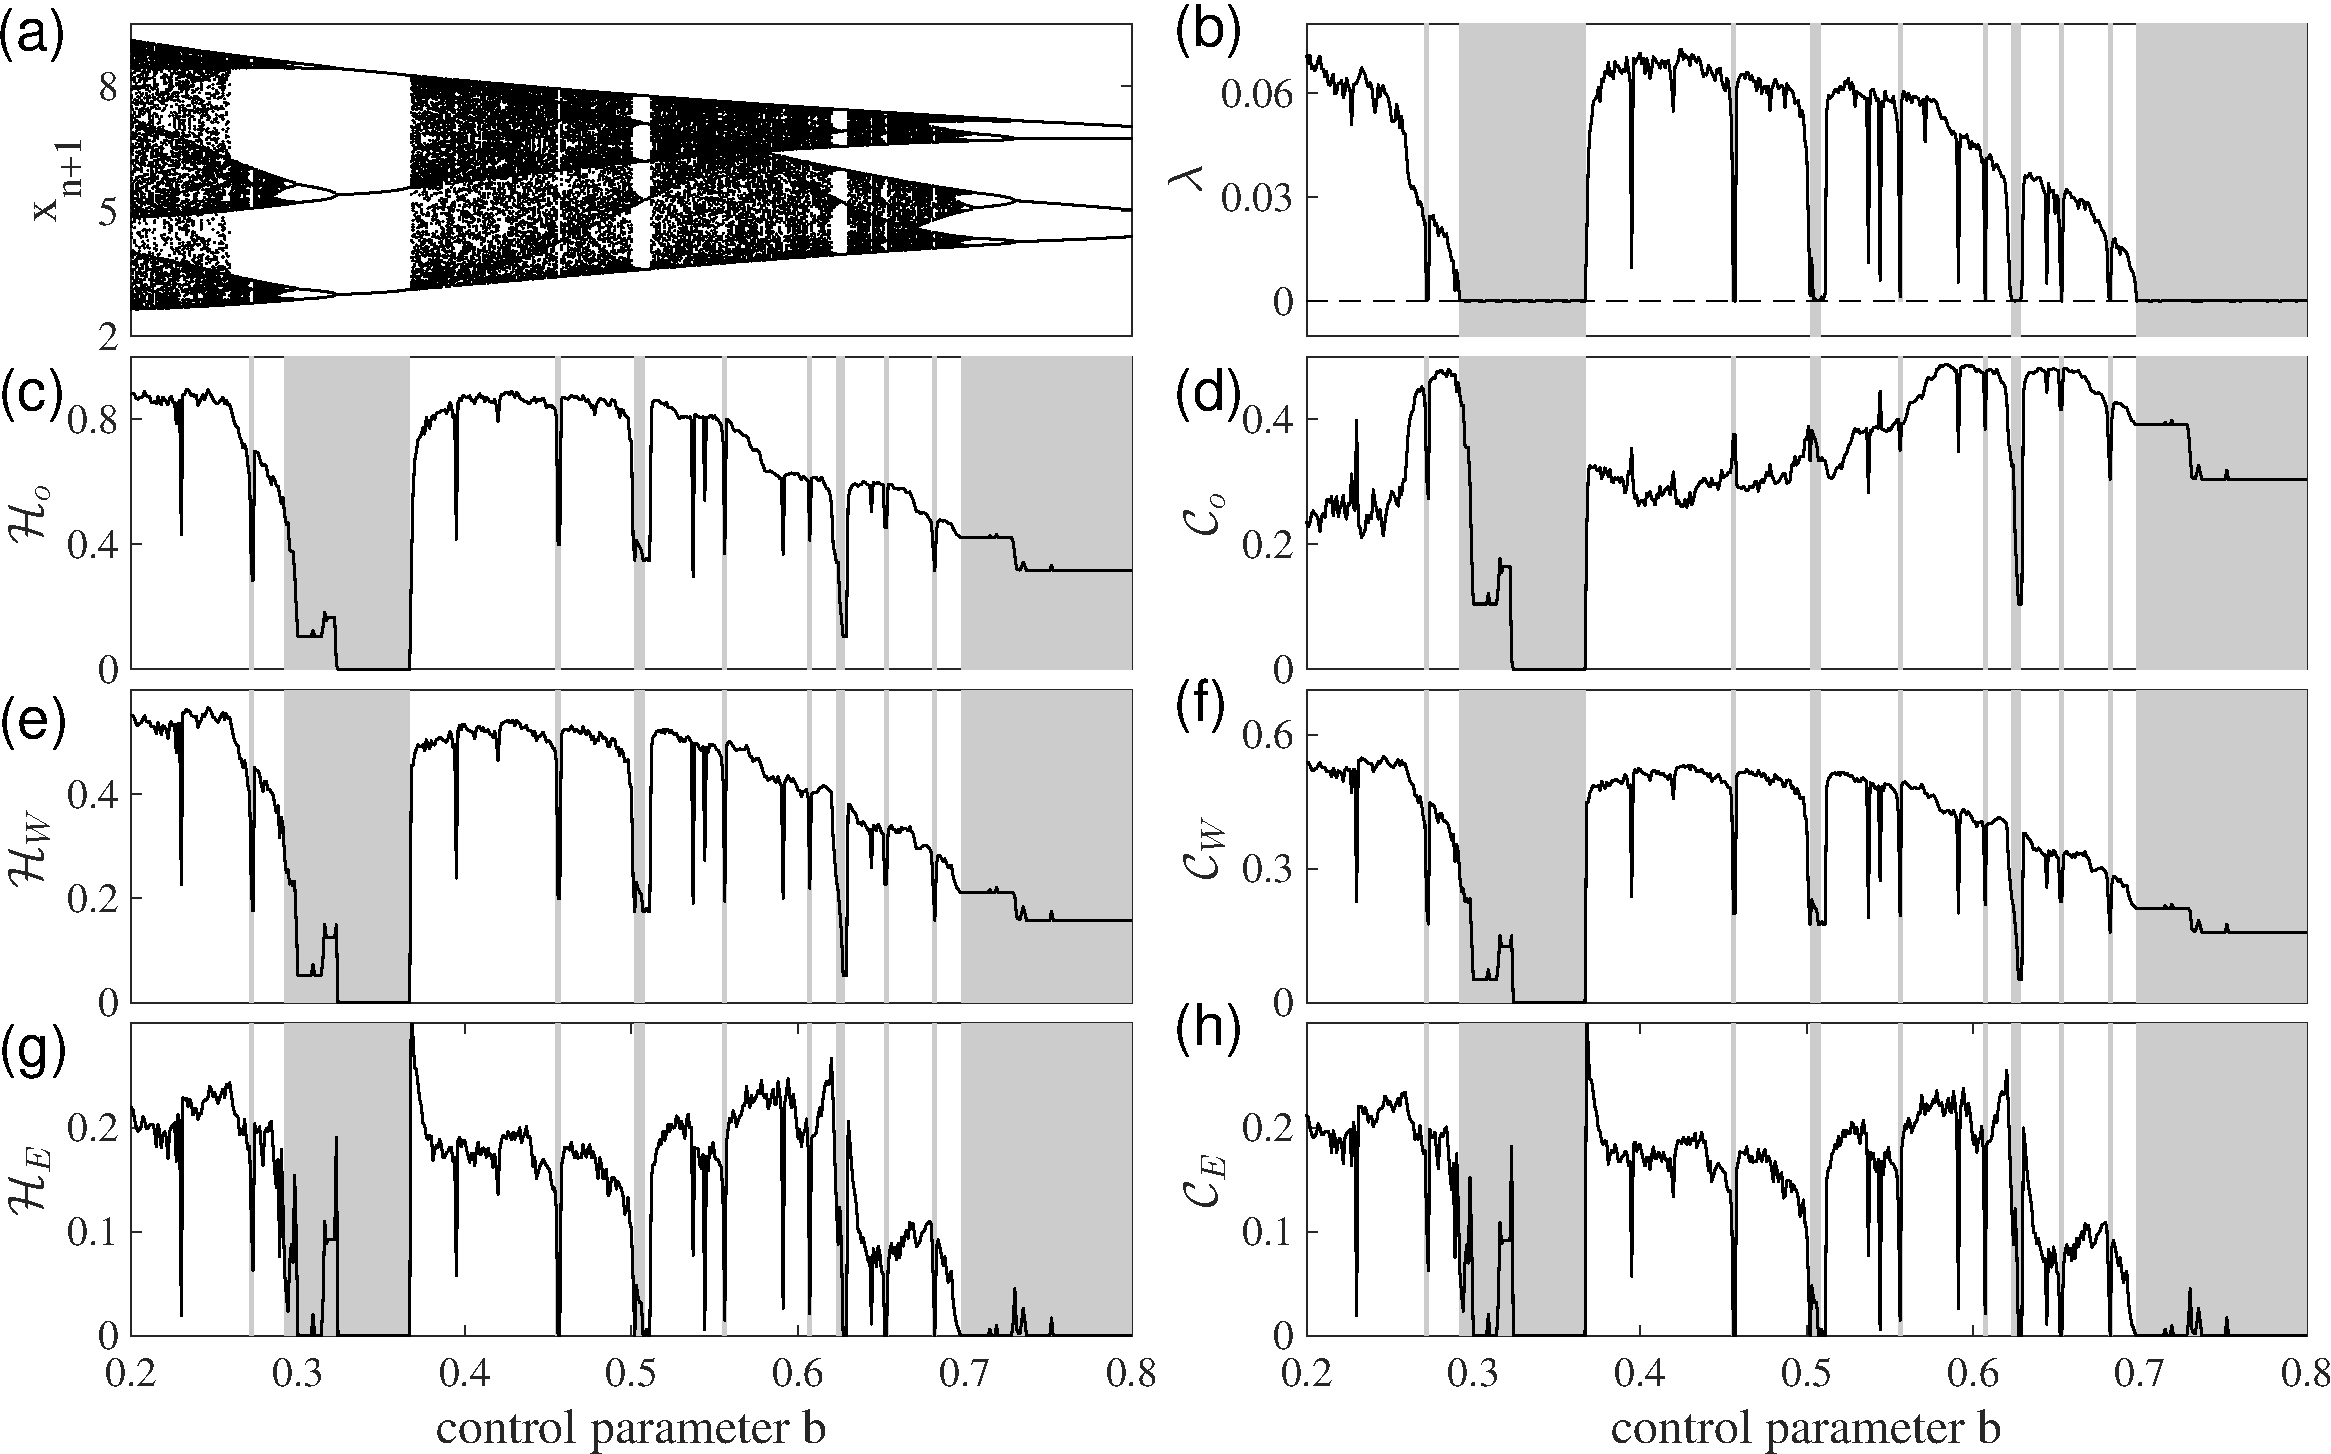
\includegraphics[width=2\columnwidth]{rosslerEntropy.pdf}
\caption{\small{Same as Fig. \ref{fig:bifurcation}, but for Poincar\'e sections of the R\"ossler system while varying the control parameter $b$ (see text for details {\color{red}and embedding dimension $D = 6$).} Panel (a) presents a bifurcation diagram based on the $x$ components of all points in the Poincar\'e sections. Panel (b) shows the largest Lyapunov exponent of the system in dependence of $b$.} \label{fig:bifurRossler}}
\end{figure*}


\section{Real-world examples} \label{sec:time}
While we have previously demonstrated the suitability of OPTN based SCMs for tracing changes in dynamical complexity for time series from deterministic dynamical systems, in the following we will use two different sets of experimental time series to demonstrate that SCMs also successfully characterize the complexity properties of real-world systems, showing distinct values for different types of dynamics. 

The first example originates from a laboratory fluid experiment of baroclinic instability which is used to study patterns of cyclones and anticyclones in the Earth's atmosphere~\cite{Read_jfm_1992,ZouEPJST2008}. Depending on the parameters of rotation rate, temperature difference, viscosity and fluid density, this experimental system exhibits a rich variety of flow regimes. In particular, we focus on the following regimes: 
\begin{enumerate}[(i)]
\item {Stable fluid (SW):} The temperature signal of the stable flow exhibits periodic oscillations as the wave drift patterns arrive at the fixed point of measurements. 
\item {Quasi-periodic 2-frequency amplitude vacillation (AV-2):} This case is identified as a 2-frequency quasi-periodic amplitude flux. The wave drift is composed of slow and regular oscillations in the temperature signal, but a fast modulation in the amplitude is also visible. AV-2 is characterized by a periodic growth and drop in wave amplitude with little change in waveform. 
\item {Quasi-periodic 3-frequency amplitude vacillation (AV-3):} For the sake of completeness, we also analyze a quasi-periodic 3-frequency amplitude vacillation time series. Unlike for the other studied cases, this time series has not been obtained from experimental results, but from a three-dimensional direct numerical simulation of the air-filled rotating baroclinic instability experiment~\cite{Read_jfm_1992}. 
\item {Modulated amplitude vacillation (MAV):} This case is identified as a low-dimensional stream, chaotically modulated and with waves of varying amplitudes. Amplitude modulation results in a complex temperature dynamics.
\end{enumerate}
{\color{red}One temperature time series of each flow regime has been measured at $2$s for periods of up to $9 \times 10^4$s. Therefore, each recording consists of $N = 45000$ data points. The examples of segmented time series have been shown in Fig. \ref{tseriesFluid} for the illustration purpose. Further details of the lower dimensional chaotic properties have been reported in \cite{Read_jfm_1992,thiel2004a}. }
\begin{figure}
	\centering 
	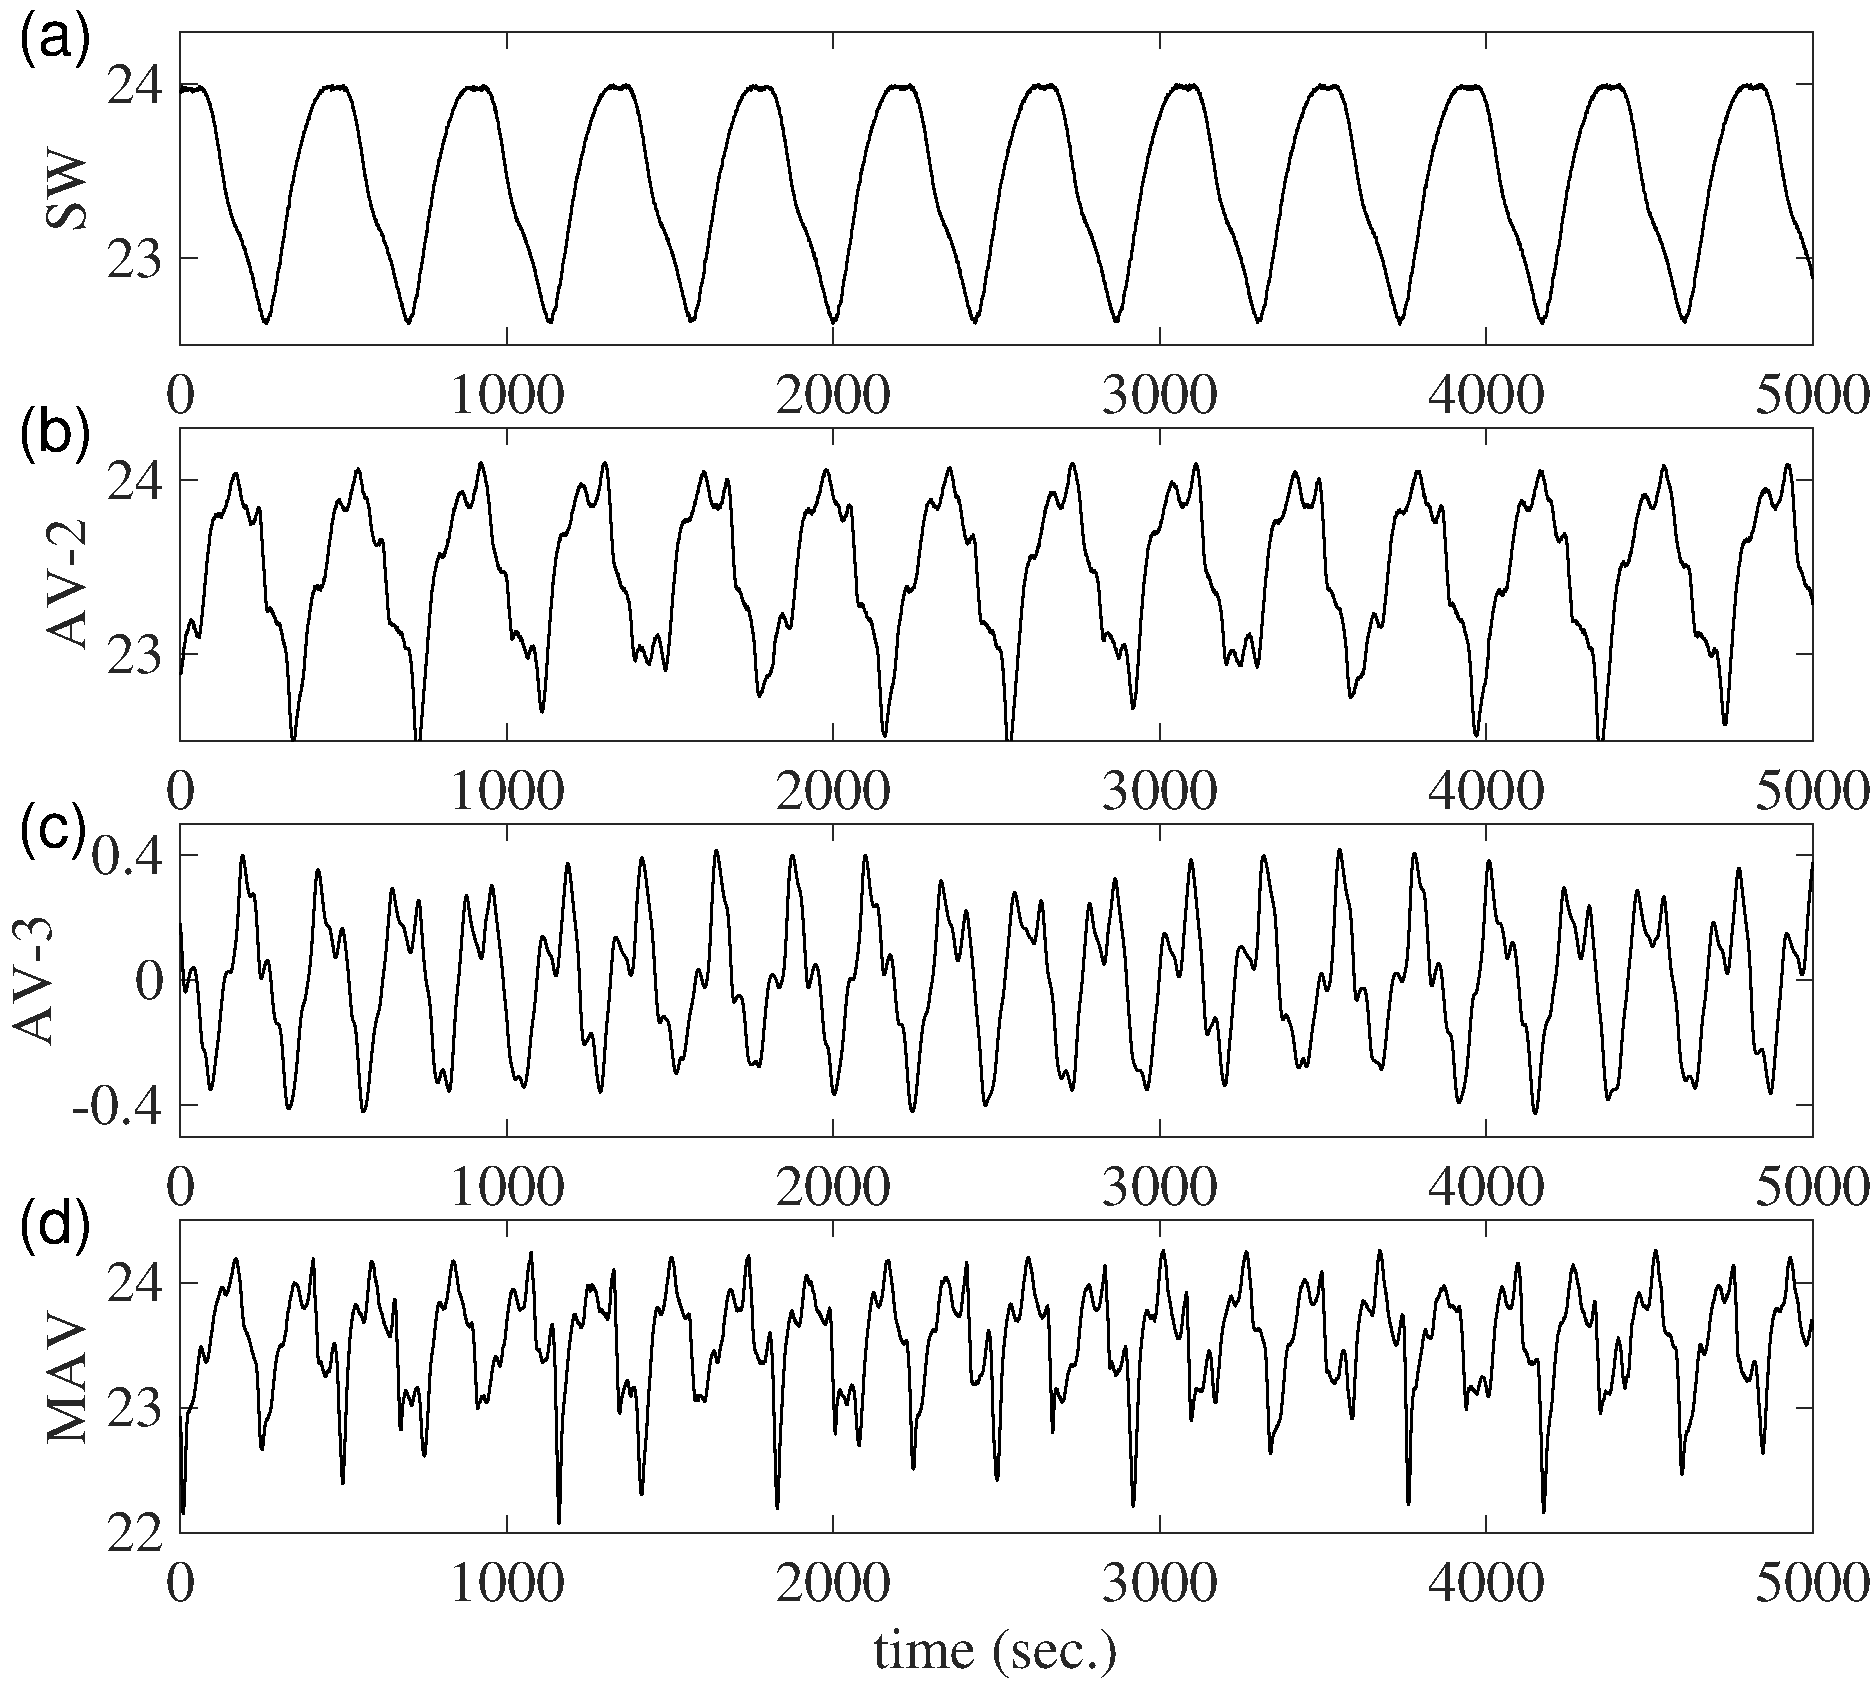
\includegraphics[width=\columnwidth]{TS_fluid.pdf}
\caption{\small{Sample segments of the temperature recordings from the flow experiment: (a) SW, (b) AV-2, (c) AV-3 and (d) MAV. The vertical axis is temperature $T$. } \label{tseriesFluid}}
\end{figure}

The second set of example time series comprises physiological signals of human electrocardiogram (ECG) recordings collected from patients from MIT-BIH Database and the Creighton University Cardiac Center \cite{GoldbergerMITBIH2000}. Heart rate variability suffering from ventricular arrhythmia presents a physiologically highly significant anomaly that is still relatively poorly understood from a dynamical system perspective, showing rich nonlinear properties \cite{smallCSF2002}. {\color{red}The ECG recordings have been measured at a 250~Hz sampling frequency for about 8.5 minutes \cite{GoldbergerMITBIH2000}. From these long term recordings, we focus on three different rhythmic states of normal sinus rhythm (SR), ventricular tachycardia (VT) and ventricular fibrillation (VF) \cite{smallCSF2002}, which have been annotated by skilled cardiologists on the basis of waveform morphology. To reduce the possible finite size effects in calculating SCMs, we choose each time series of at least $10000$ time points. In consequence, out of 18 different patients we obtain 14 time series showing sinus rhythm (SR) prior to onset of arrhythmia, 12 records of VT and 17 records of VF. After the annotations, each time series may have different length, ranging from $14600$ to $159600$ data points in SR, $16000\sim 132000$ in VT, and $14500 \sim 124000$ in VF. We do not apply any preprocessing to the data, except checking the length requirements. We show some sections of time series of each case in Fig. \ref{tseriesECG}. } 
\begin{figure}
	\centering 
	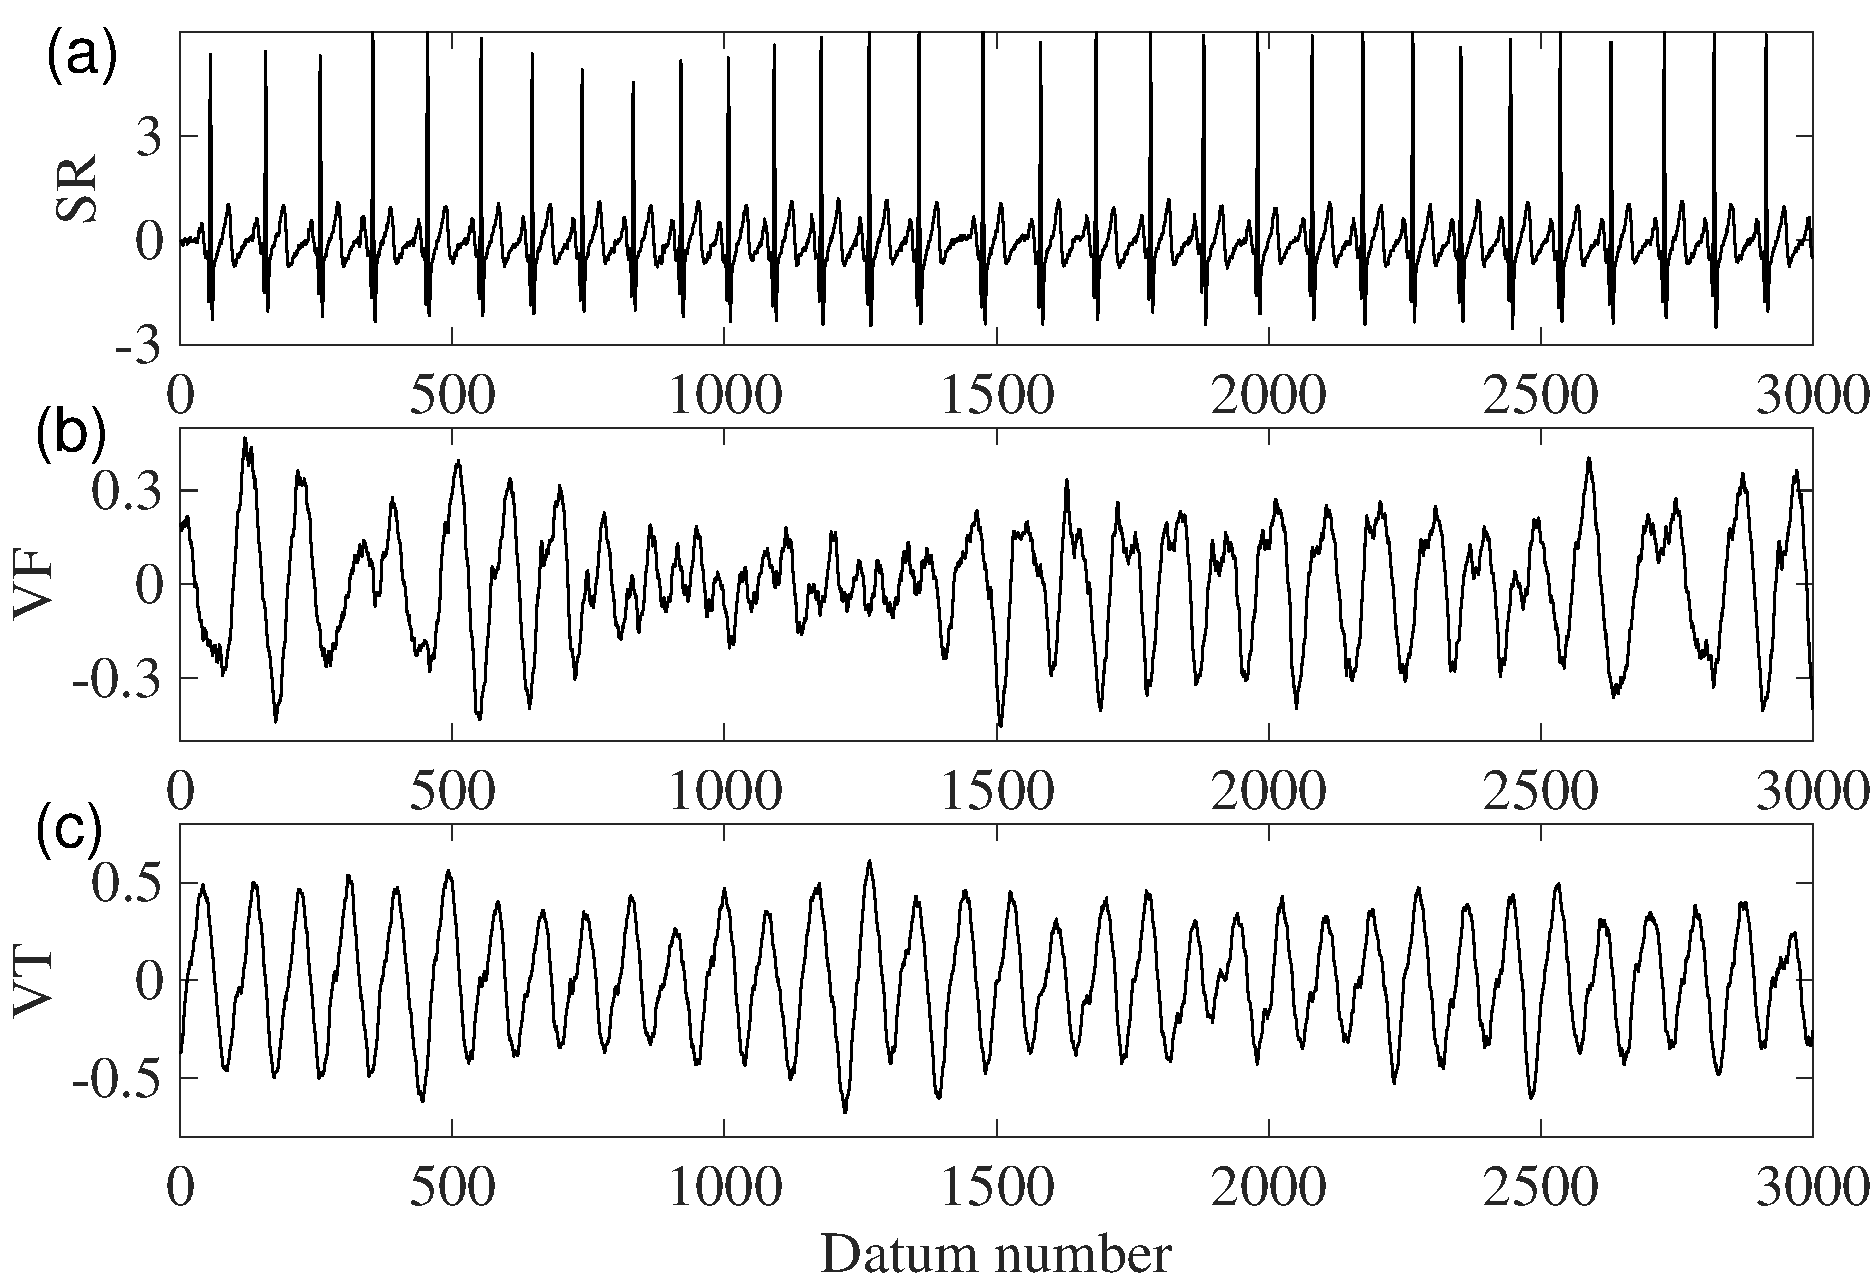
\includegraphics[width=\columnwidth]{TS_ECG.pdf}
\caption{\small{Three representative ECG recording sections (randomly chosen from different rhythmic states): (a) sinus rhythm (SR), (b) VF and VT. The horizontal axis of each panel is the datum number (at 250 Hz) and the vertical axis is ECG surface voltage (in milli-volts). } \label{tseriesECG}}
\end{figure}

For choosing the embedding parameters for both sets of example time series, we follow the suggestions from earlier studies~\cite{ZouEPJST2008,smallCSF2002}. Although we are facing the inevitable presence of nonstationarity and noise in the experimental data, we have verified that the following results do not change {\color{red}qualitatively} while the embedding parameters are varied. In particular, we have treated the embedding dimension as a free parameter which has been varied in the range of $D = 2, 3, \ldots, 6$, while the embedding delay $\tau$ has been {\color{red} determined by the first zero of the autocorrelation function \cite{Kantz97}. In the case of temperature time series from the fluid experiments, $\tau_{1} = 110$ time steps (data points) for SW, AV-2 and AV-3, while $\tau_{2} = 60$ for MAV,  which have been consistent with the literature \cite{Read_jfm_1992,thiel2004a}.} For the ECG time series, we consistently use an embedding delay of $\tau = 5$ time steps as suggested in \cite{smallCSF2002}. The results have been averaged over all subjects. 

In both sets of time series, the OPTN based SCMs enhance our understanding of the underlying nonlinear system, which can be seen from the results summarized in Figs. (\ref{fig:fluid}, \ref{fig:ecg}). For the fluid data (Fig.~\ref{fig:fluid}), $\mathcal{H}_O$, $\mathcal{H}_W$, $\mathcal{C}_W$, $\mathcal{H}_E$ and $\mathcal{C}_E$ all show consistent changes of the complexity and entropy values between stable wave solution (SW), quasi-periodic 2-frequency amplitude vacillation (AV-2), quasi-periodic 3-frequency amplitude vacillation (AV-3) and chaotic modulated amplitude vacillation (MAV). Specifically, the complexity of these four cases has the following order: SW has the lowest complexity since it shows periodic oscillations with trivial recurrence, while MAV has the highest complexity since it presents chaotically modulated amplitude vacillation. Quasiperiodic states exhibit intermediate complexity values since these two cases have non-trivial recurrences while still featuring a certain degree of regularity. In our case, AV-3 presents a higher complexity than AV-2, which should however be interpreted with care since the AV-2 series originates from an experiment, while the AV-3 series has been taken from a numerical simulation of the same system (hence, there may be a certain level of observational noise present in AV-2 but not in AV-3). The order of complexity values between periodic, quasiperiodic and chaotic solutions still holds for $\mathcal{C}_O$, but the corresponding values become very similar. In particular, it becomes hard for $\mathcal{C}_O$ to identify the difference between AV-2 and AV-3. 
\begin{figure*}
	\centering 
	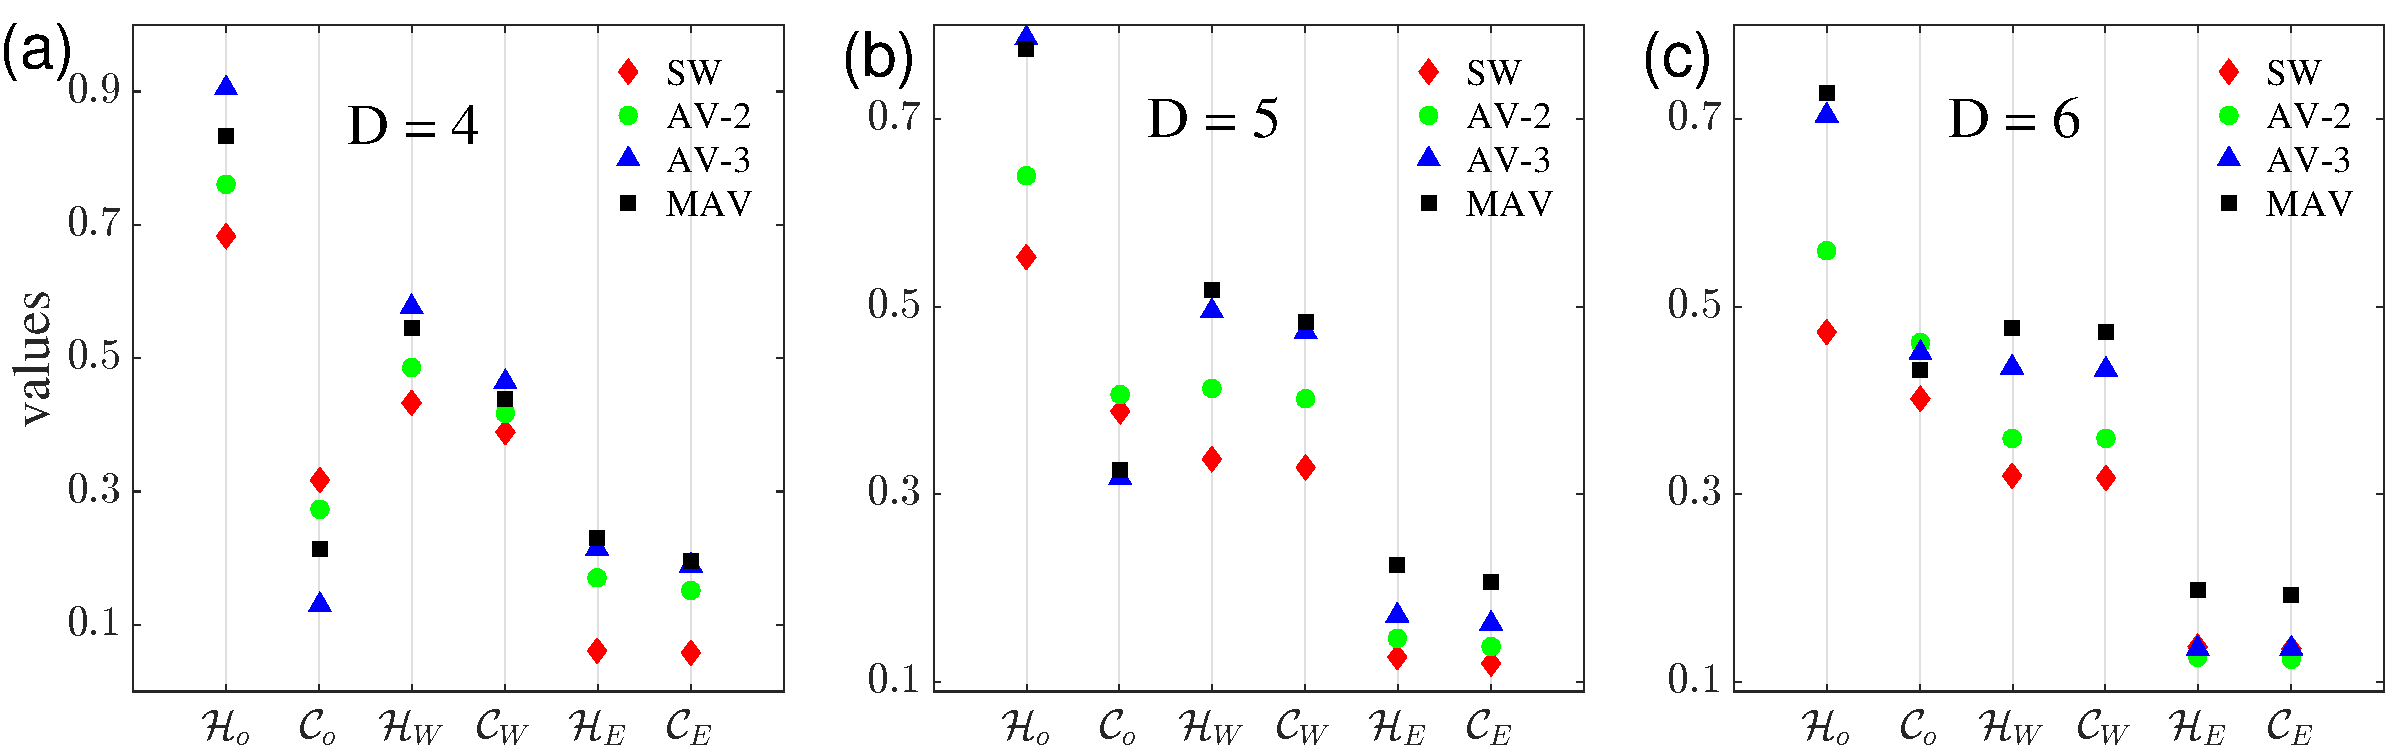
\includegraphics[width=2\columnwidth]{fluidExample.pdf}
\caption{\small{OPTN based entropy and SCM characteristics for experimental fluid data, which are shown for embedding dimensions of $D = 4, 5, 6$. In all subfigures, stable wave (SW, $\blacklozenge$), quasiperiodic 2-frequency amplitude vacillation (AV-2, $\bullet$), quasiperiodic 3-frequency amplitude vacillation (AV-3, $\blacktriangle$) and chaotic modulated amplitude vacillation (MAV, $\blacksquare$) are distinguished. } \label{fig:fluid}}
\end{figure*}

Qualitatively similar results are obtained for the ECG recordings, as shown in Fig.~\ref{fig:ecg} for three different embedding dimensions. Generally speaking, different ECG recordings exhibit remarkably distinct complexity values since the ensemble medians are well separated between different time series groups of SR, VF and VT as shown by the box plots in Fig. \ref{fig:ecg}. More specifically, SR recordings show very pronounced the highest median of $\mathcal{H}_O$, $\mathcal{H}_W$, $\mathcal{C}_W$, $\mathcal{H}_E$ and $\mathcal{C}_E$, reflecting the existence of significant spectral power in a rather broad frequency band between 50 and 100 beats/min in the signals \cite{smallCSF2002}. On the other hand, the complexity of VT has the smallest value, even lower than for the case of VF. Unlike the other five measures, we note, however, that SR shows the smallest median values of $\mathcal{C}_O$ while VT has the largest values (Fig. \ref{fig:ecg}(b)). 

 {\color{red}Meanwhile, we find mild dependence of the discriminatory power of $\mathcal{C}_O$ and $\mathcal{C}_W$ on the embedding dimension $D$. In particular, in the case of $D=6$ the median values of $\mathcal{C}_O$ of VF are comparable to that of VT (Fig.~\ref{fig:ecg}(b)). On the other hand for $D=4$, the median values of $\mathcal{C}_W$ are all comparable for SR, VF and VT (Fig.~\ref{fig:ecg}(d)). This insufficiency of $\mathcal{C}_O$ and $\mathcal{C}_W$ due to embedding may be explained by the fact that $\mathcal{C}_O$ takes only static pattern frequencies into account, while $\mathcal{C}_W$ considers dynamic pattern transitions, which may therefore not be able to properly distinguish subtle differences reflected in the temporal order of patterns. In contrast, $\mathcal{C}_E$ considers both individual pattern frequencies and dynamic pattern transition frequencies. } 
\begin{figure*}
	\centering 
	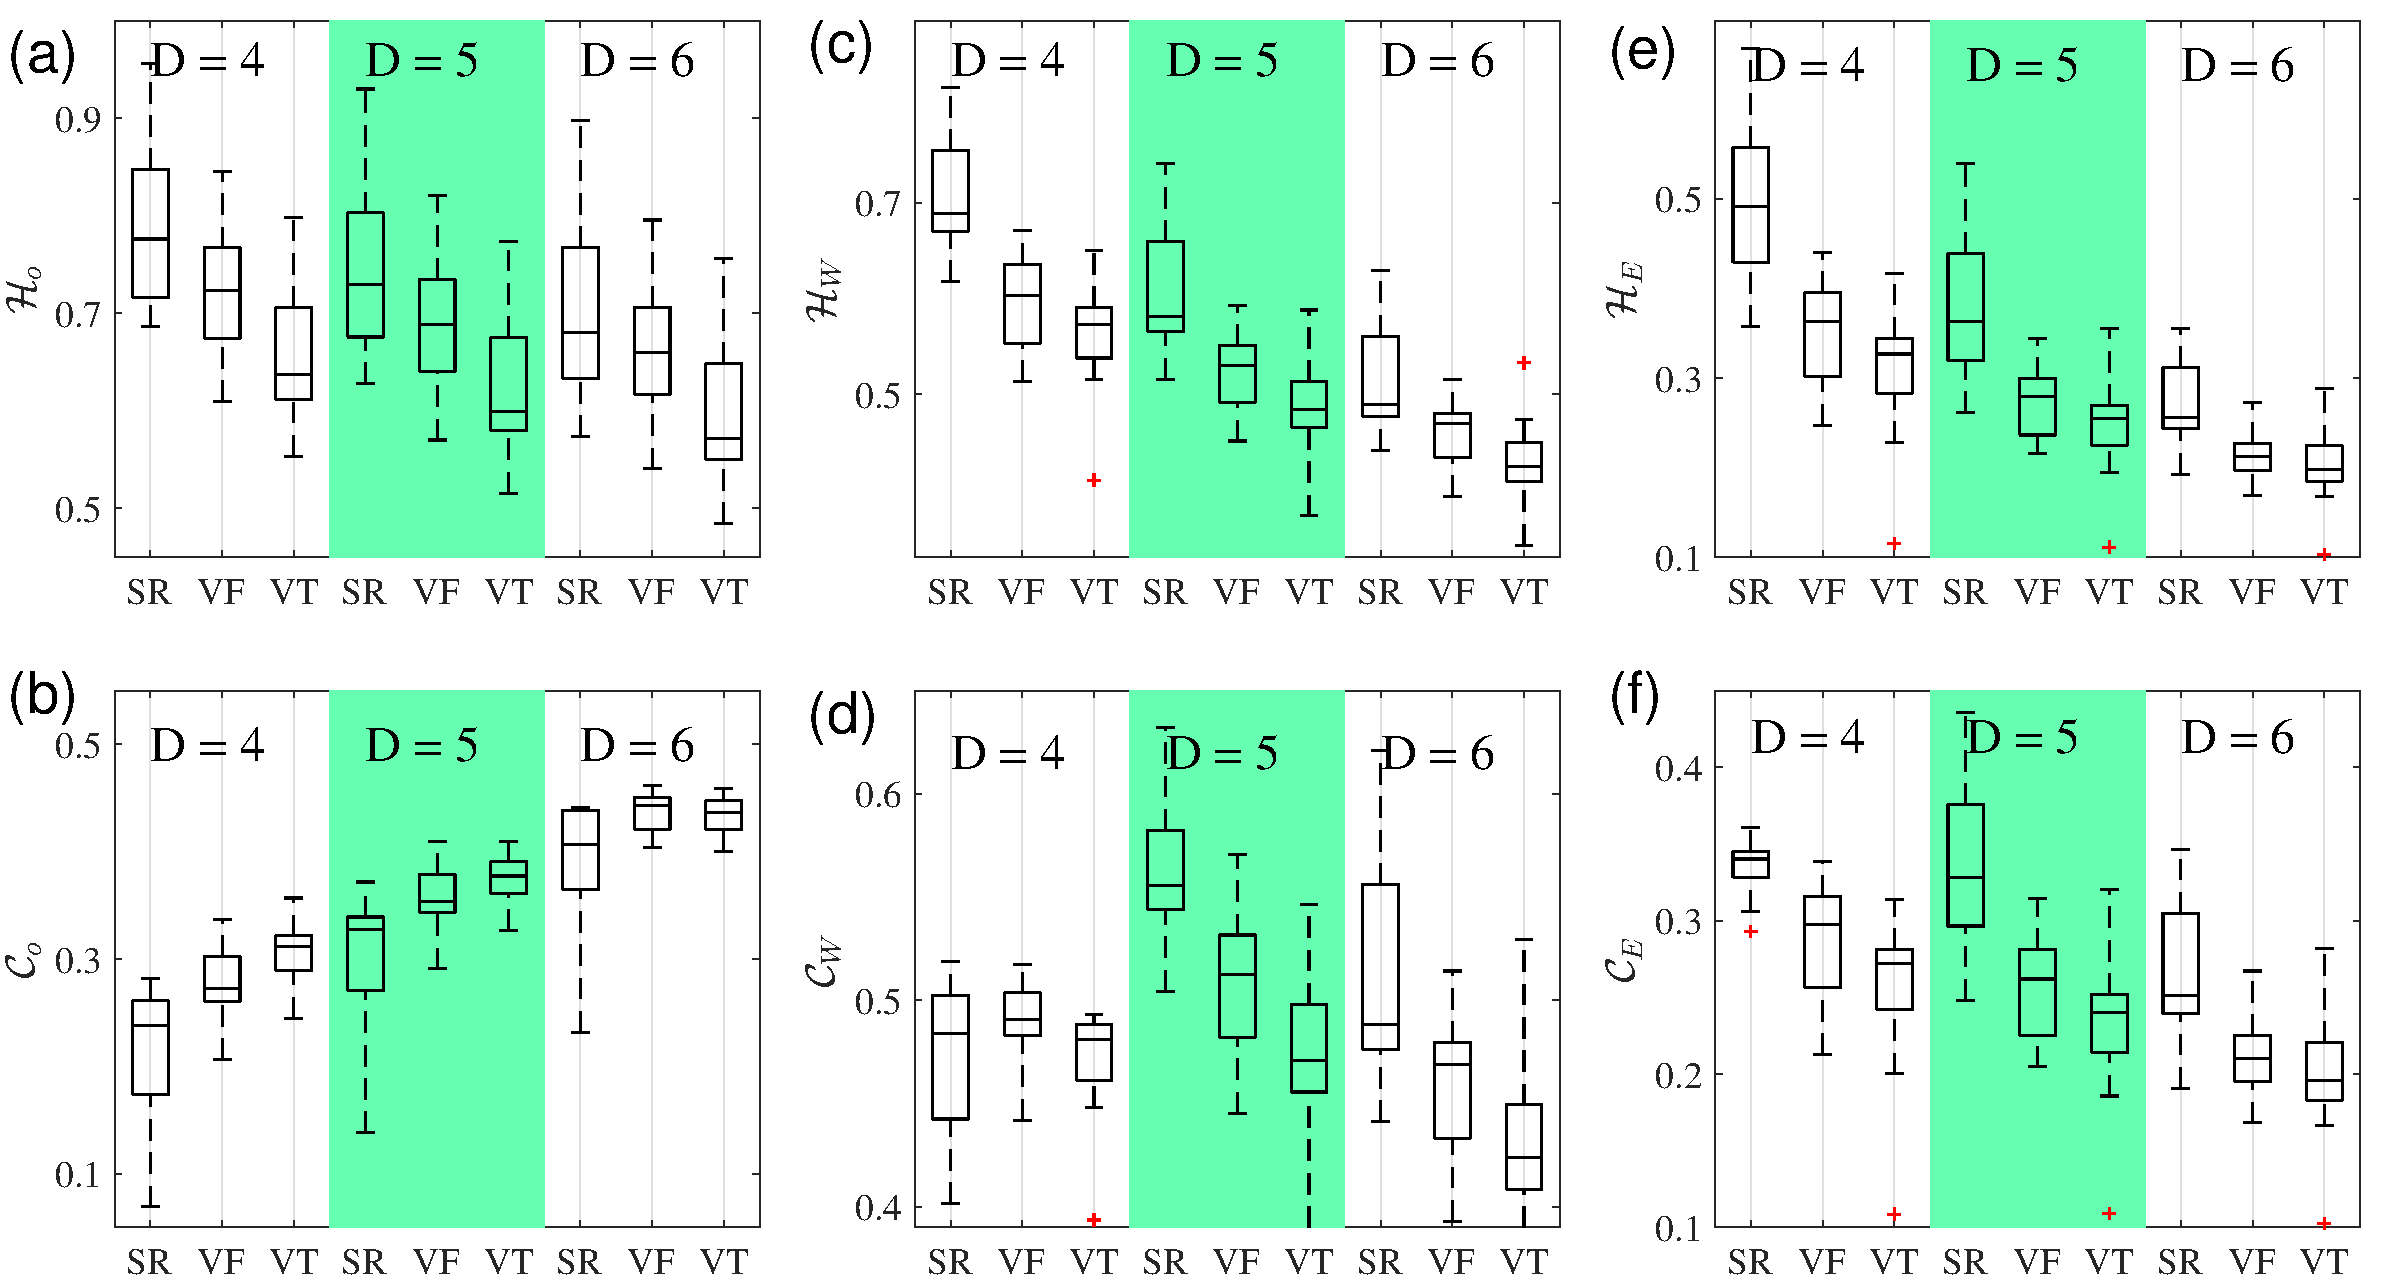
\includegraphics[width=2\columnwidth]{ecgExample.pdf}
\caption{\small{Box plots for OPTN based entropy and SCM characteristics for human ECG recordings, showing well separated medians for each subject group SR, VF and VT. Entropy and SCM scores are shown for embedding dimensions of $D = 4, 5, 6$. } \label{fig:ecg}}
\end{figure*}



\section{Conclusions} \label{sec:con}
In summary, we have proposed to expand the traditional ordinal pattern frequency analysis by also including ordinal pattern transitions, thereby generalizing existing statistical complexity measures for nonlinear time series analysis. The pattern transition properties encoded in the underlying time series networks allow to gain insights beyond those provided by the celebrated permutation entropy method which relies on the pattern frequencies only. Therefore, this study presents another case showing the usefulness of applying ordinal pattern transition networks for time series analysis \cite{ZouPR2018}. 

We have suggested two slightly different ways to incorporate the effects of pattern transitions in statistical complexity measures, which are based on (i) a globally normalized transition matrix and (ii) a node-wise normalized transition matrix. Here, the complexity measure based on the node-wise normalized matrix combines both, individual pattern frequencies and the frequencies of transitions among patterns. We have shown that the associated two new statistical complexity measures characterize the complexity properties of deterministic chaos successfully and clearly highlight deterministic-chaotic dynamics in the corresponding complexity--entropy planes (Fig.~\ref{fig:CElogistic}). This finding helps to obtain an improved complexity analysis for time series of both, deterministic chaos and stochastic systems, fostering their better discrimination. However, further more systematic numerical performance tests employing different types of dynamical systems are required to provide compelling evidence for distinctions between different types of dynamics beyond the cases presented in the current work~\cite{BorgesAMC2019,RossoPRE2007}. While this opens several opportunities for follow-up research, we have already demonstrated here the practical usefulness of our improved SCMs by employing this framework to time series of experimental fluid flows and ECG recordings, showing {\color{red} statistically significant discrimination} for different cases. 

Some open problems also com	mon to other nonlinear time series analysis methods remain to be further addressed, for example, the dependence of reliable estimates of SCMs on the available time series length. {\color{red}For reliable estimations of traditional entropy $\mathcal{H}_O$ and SCM $\mathcal{C}_O$, the length $N > 5 D!$ has been largely suggested \cite{BandtPRL2002,AmigoPTRSA2014}. However, even longer length is required for the newly proposed SCMs based on transition frequencies because the transition matrix has the dimension $D!\times (D! - 1)$ if self loops are excluded. This should not be a big problem when working with time series from numerical models provided with the rapid increased computing power nowadays. } For time-discrete dynamical systems like chaotic maps, one may easily use longer data series, which however does not seem to improve the estimates very much due to the accumulation of effects due to a limited numerical precision (Fig.~\ref{fig:transient}). {\color{red} The dependence of the new SCMs on the length $N$ becomes crucial for experimental time series studies. One of more interesting problems is to understand the extra information of transition probability based complexity measures since linear correlations have been found for $\mathcal{C}_{E}$ and small entropy $H$, which are expected for a large number of patterns, i.e., $N = D!$ for high embedding $D$ or equivalently $N = D! \times (D!-1)$ transitions. } For continuous systems, together with the embedding parameters, the sampling frequency is another important characteristic which needs to be further explored. Moreover, the generalization of our approach from univariate to bivariate time series analysis shall be further discussed. We noticed that this aspect has remained a largely untouched subject for statistical complexity analysis so far, while it presents an interesting task to show the dependence of complexity on interaction. {\color{red} We may integrate some of the traditional network topological statistical measures of higher order into the SCMs, for instance, clustering coefficients or path lengths, which have been widely discussed to characterize the dynamical properties of the system generating the time series at hand \cite{ZouPR2018}.} We outline further work on the aforementioned topics as subjects of future research. 

\section*{Acknowledgements}
Parts of this work have been financially supported by the National Natural Science Foundation of China (grant no. 11872182, 11835003, 11875132, 61973086), the Natural Science Foundation of Shanghai (grant no. 18ZR1411800). JZ and YZ further acknowledge support by the Shanghai Municipal Science and Technology Major Project (grant no. 2018SHZDZX01) and ZJ Lab. The authors thank J. B. Borges and O. A. Rosso for sharing algorithms for computing $\mathcal{C}_{min}$ and $\mathcal{C}_{max}$. 

\section*{Data Availability Statement}
The fluid data that support the findings of this study are available from the corresponding author upon reasonable request. The ECG data that support the findings of this study are openly available in {\tt https://www.physionet.org} from MIT-BIH Database and the Creighton University Cardiac Center \cite{GoldbergerMITBIH2000}. 


\bibliography{ref_Zou,ref_Donner}

\end{document}
